% -*- coding: utf-8 -*-

\documentclass[a4paper,dvipdfmx]{jsarticle}
\usepackage{ascmac,alltt,txfonts,url}

\usepackage[dvipdfmx]{graphicx}
\usepackage{here}
\usepackage{fancyvrb}

\renewcommand{\ttdefault}{cmtt}
\renewcommand{\figurename}{図} 
\renewcommand{\tablename}{表} 
\DeclareMathAlphabet{\mathtt}{OT1}{cmtt}{m}{n}
\SetMathAlphabet{\mathtt}{bold}{OT1}{cmtt}{m}{n}
\setlength{\oddsidemargin}{0cm}
\setlength{\evensidemargin}{0cm}

\makeatletter

\newdimen\@mojihaba
\settowidth{\@mojihaba}{あ}

\def\tokushu#1{%
\def\tokushutitle{#1}%
\gdef\articleHeader{\hbox to\textwidth{\rule{3\@mojihaba}{1mm}%
\hbox{\small\bf\hskip1mm \tokushutitle}\leaderfill}}
}

\newdimen \JQ	\JQ .259817mm	%%%	\JQ/\Q = 10pt/9.62216pt
\newdimen \Q	\Q  .25mm	%%%	Quarter of 1mm

\def\JarticleHeader{\rule{\textwidth}{1mm}}%
\def\JarticleTitle{{\huge\bf\@title}}
\def\JarticleAuthor{\large\begin{tabular}[t]{@{}l}\@author\end{tabular}}
\newbox\@temptitlebox

\def\verse{\let\\=\@centercr 
 \list{}{\itemsep\z@ \itemindent -1.5em\listparindent \itemindent 
 \rightmargin\leftmargin\advance\leftmargin 1.5em}\item[]}
\let\endverse\endlist
\def\quotation{\list{}{\listparindent 1.5em
 \itemindent\listparindent
 \rightmargin\leftmargin \parsep 0pt plus 1pt}\item[]}
\let\endquotation=\endlist
\def\quote{\list{}{\rightmargin\leftmargin}\item[]}
\let\endquote=\endlist
\def\abstquotation{\list{}{\listparindent 1.5em
 \itemindent\listparindent
 \leftmargin 5mm
 \rightmargin\leftmargin \parsep 0pt plus 1pt}\item[]}
\let\endabstquotation=\endlist
\def\quote{\list{}{\rightmargin\leftmargin}\item[]}
\let\endquote=\endlist

\global\def\@maketitle{\newpage \null
\hbox{\vbox to193.5\Q{\baselineskip=10mm % 193.5\Q = 9*\baselineskip
\begin{flushleft}
\JarticleHeader
% following extra vskip together with baselineskip(10mm) will produce
% appropriate 10mm/6mm gap between the rule and title
% This assumes that title is typeset with 28Q(7mm) font, and baseline
% is set 1mm above the bottom of the font.
\setbox\@temptitlebox\hbox{JarticleTitle}\ifdim\wd\@temptitlebox>\textwidth\vskip2mm\else\vskip6mm\fi
\leftskip=5mm
\JarticleTitle
\vskip6mm % to leave 10mm gap between title and author
\JarticleAuthor
\end{flushleft}\vfil}}
%\JEabstInsert
  \begin{small}
    \begin{abstquotation}
      \Jabstcontent
    \end{abstquotation}
  \end{small}
}

\long\def\Jabstract#1{\global\long\def\Jabstcontent{\noindent\ignorespaces #1}}
\def\Jabstcontent{\relax}

\makeatother

\usepackage{fancyhdr}
\pagestyle{fancy}
\lhead{基本実験}
\rhead{}
\rhead{\thepage{}}
\cfoot{}
\renewcommand{\headrulewidth}{0.5pt}
\pagestyle{fancy}

\Jabstract{%
\\
かんたんな実験を通じてFPGAでのハードウェア作りの基礎力を手に入れましょう.
}

\begin{document}

\title{基本実験}
\author{}
\date{2019年 1月14日~~第3.0版}
\maketitle

\section{はじめに}
いくつかの簡単なHDLコードを書いて,FPGAでのハードウェア作りの基礎力を手に入れましょう.実際にHDLコードを書き,シミュレーションして,実機動作を確認することは,より複雑なハードウェアを設計するための第一歩です.

\section{ILAを使ってFPGA内部の信号を観測する}
FPGAは,FPGAの中で回路がどのように動作しているのかを知るためのILA(Internal Logic Analyzer)という仕組みを持っています.実験コードを書きはじめる前に,このILAの使い方を学んでみましょう.

\subsection{LチカでILAの動作を学ぶ}
三度目の登場ですが,LチカでILAの動作を学びましょう.第4章で利用した\verb|project_2|を使用します.

\subsection{準備}
ILAを使ってデバッグするために,topモジュールのソースコードを次のように書き変えてください.

\begin{figure}[H]
\begin{quote}
\begin{Verbatim}[frame=single, numbers=left, baselinestretch=0.8]
 library ieee;
 use ieee.std_logic_1164.all;
 use ieee.numeric_std.all;

 entity top is
    Port ( clk   : in std_logic;
           reset : in std_logic;
           led   : out std_logic
         );
 end top;

 architecture RTL of top is
  
  attribute mark_debug : string; -- (1) 追加
  signal counter : unsigned(31 downto 0) := (others => '0');
  attribute mark_debug of counter : signal is "true"; -- (2) 追加

 begin

  -- カウンタの3bit目をledに接続(実機では23bit目を使った)
  led <= std_logic(counter(3));

  process(clk) -- クロックの変化で動作するプロセス
  begin
    if rising_edge(clk) then -- クロックの立ち上がりであれば
      if reset = '1' then
        counter <= (others => '0');
      else
        counter <= counter + 1; -- カウンタをインクリメント
      end if;
    end if;
  end process;

 end RTL;
\end{Verbatim}
\end{quote}
\caption{ILA実験用に変更したリストの例}
\end{figure}

(1)と(2)が追加ポイントです.(1)で\verb|mark_debug|というattributeを利用することを宣言し,(2)でcounterに\verb|mark_debug|というattributeを付与しています.attributeは,ツールに対する指示子です.Vivadoでは,\verb|mark_debug|を付与した信号はデバッグ対象の可能性があるとして特別扱いします.

コードが準備できたら,一度合成してピン配置まで終わらせてしまいましょう.

 \begin{figure}[H]
  \begin{center}
   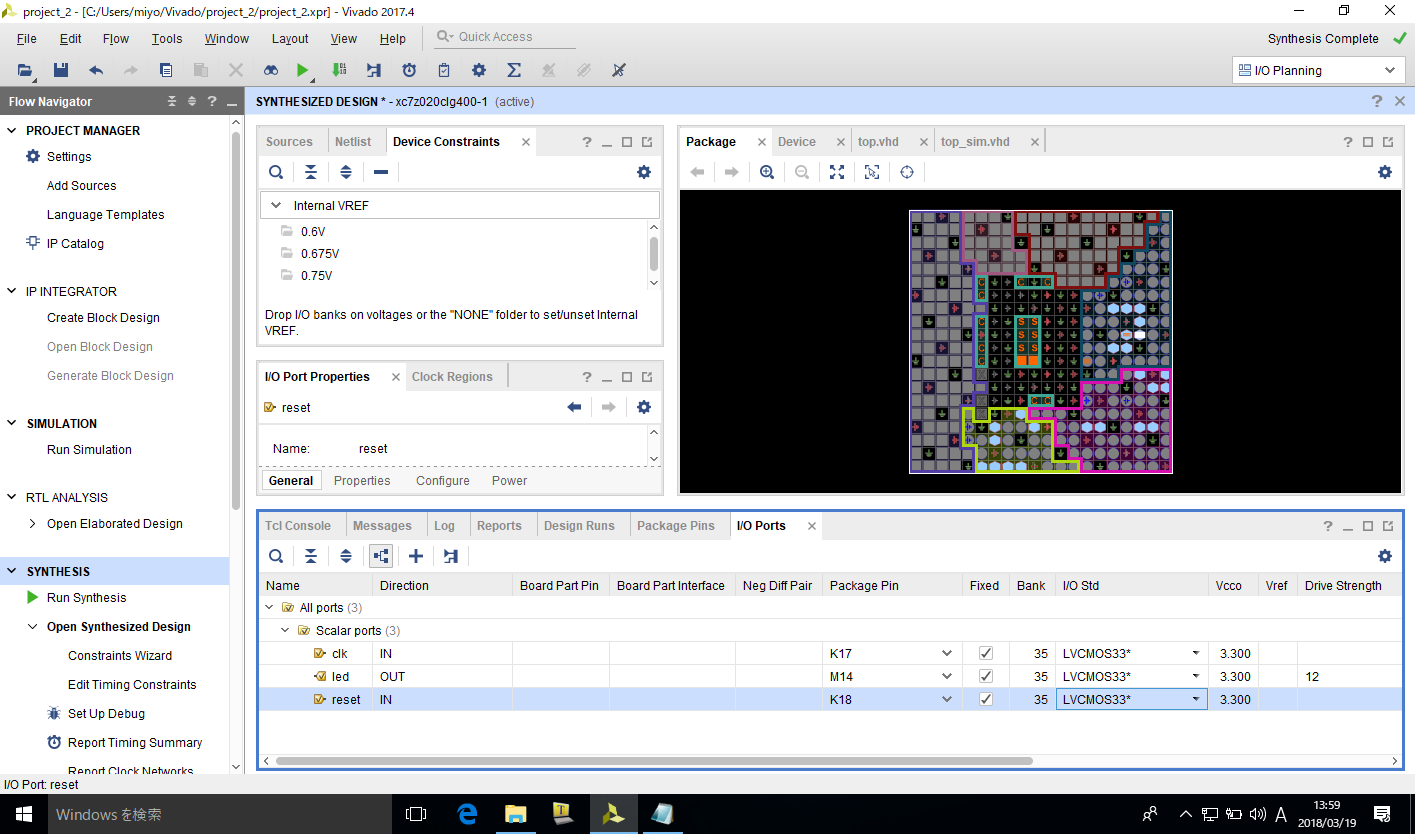
\includegraphics[width=.8\textwidth]{chapter05_figures/VirtualBox_Windows10_19_03_2018_13_59_41.png}
  \end{center}
  \caption{I/O Planningでclk,reset,ledのピン配置を決定する}
 \end{figure}


\subsection{ILAのセットアップと利用方法}
準備ができたらILAを追加して,その動作の様子を確認してみましょう.

 \begin{figure}[H]
  \begin{center}
   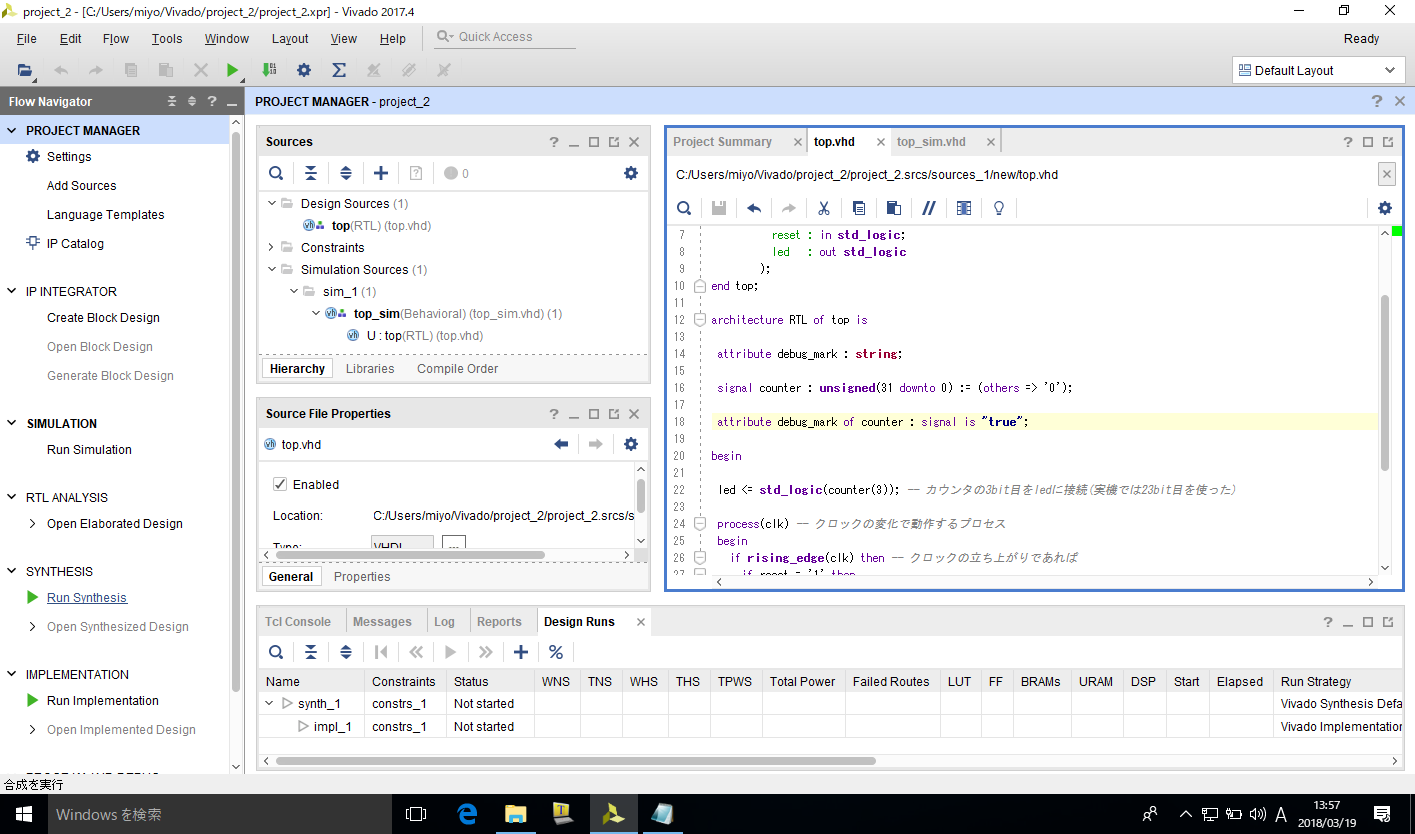
\includegraphics[width=.8\textwidth]{chapter05_figures/VirtualBox_Windows10_19_03_2018_13_57_01.png}
  \end{center}
  \caption{一度合成する}
 \end{figure}

 \begin{figure}[H]
  \begin{center}
   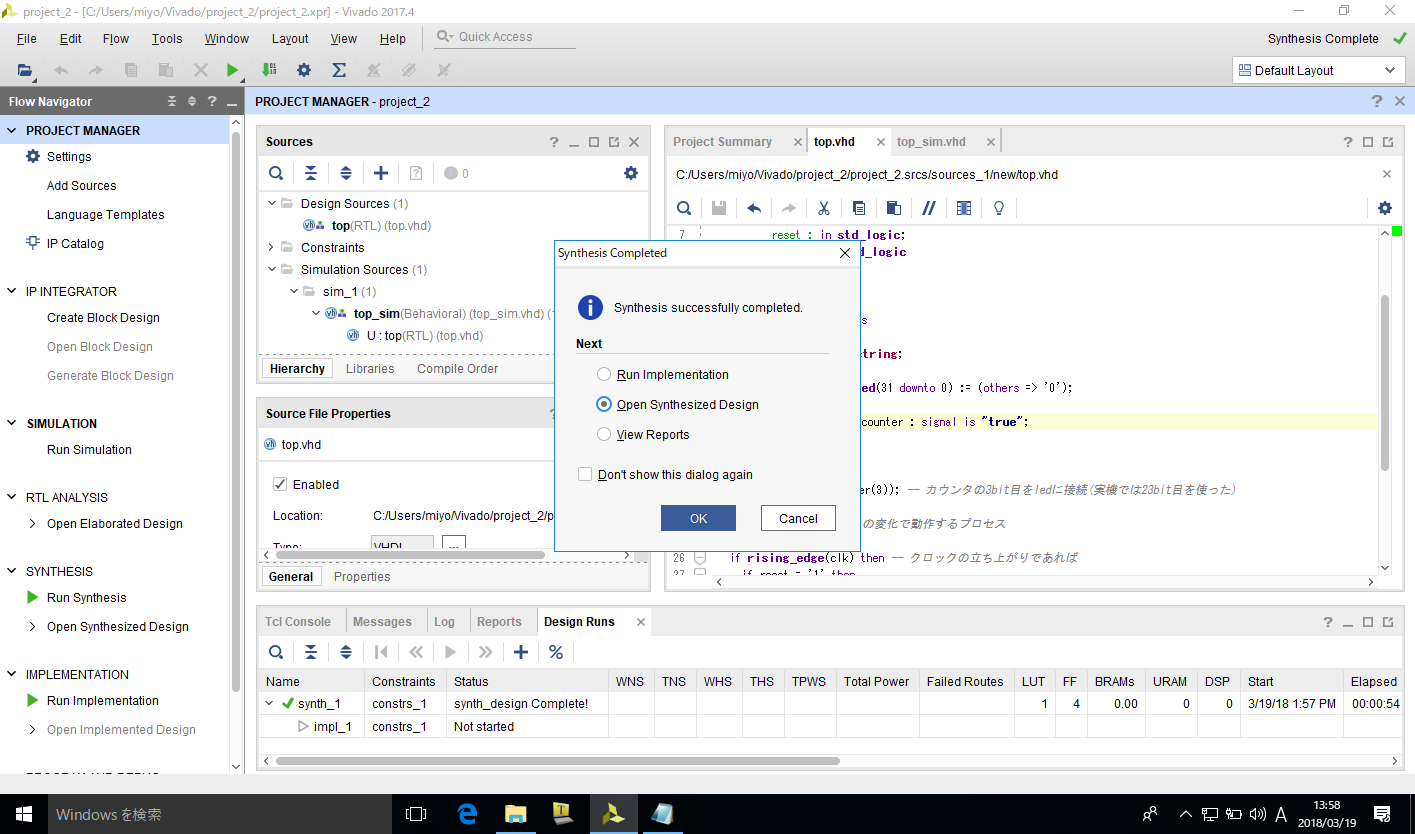
\includegraphics[width=.8\textwidth]{chapter05_figures/VirtualBox_Windows10_19_03_2018_13_58_37.png}
  \end{center}
  \caption{合成が終わったらOpen Synthesized Designで合成結果を開く}
 \end{figure}

 \begin{figure}[H]
  \begin{center}
   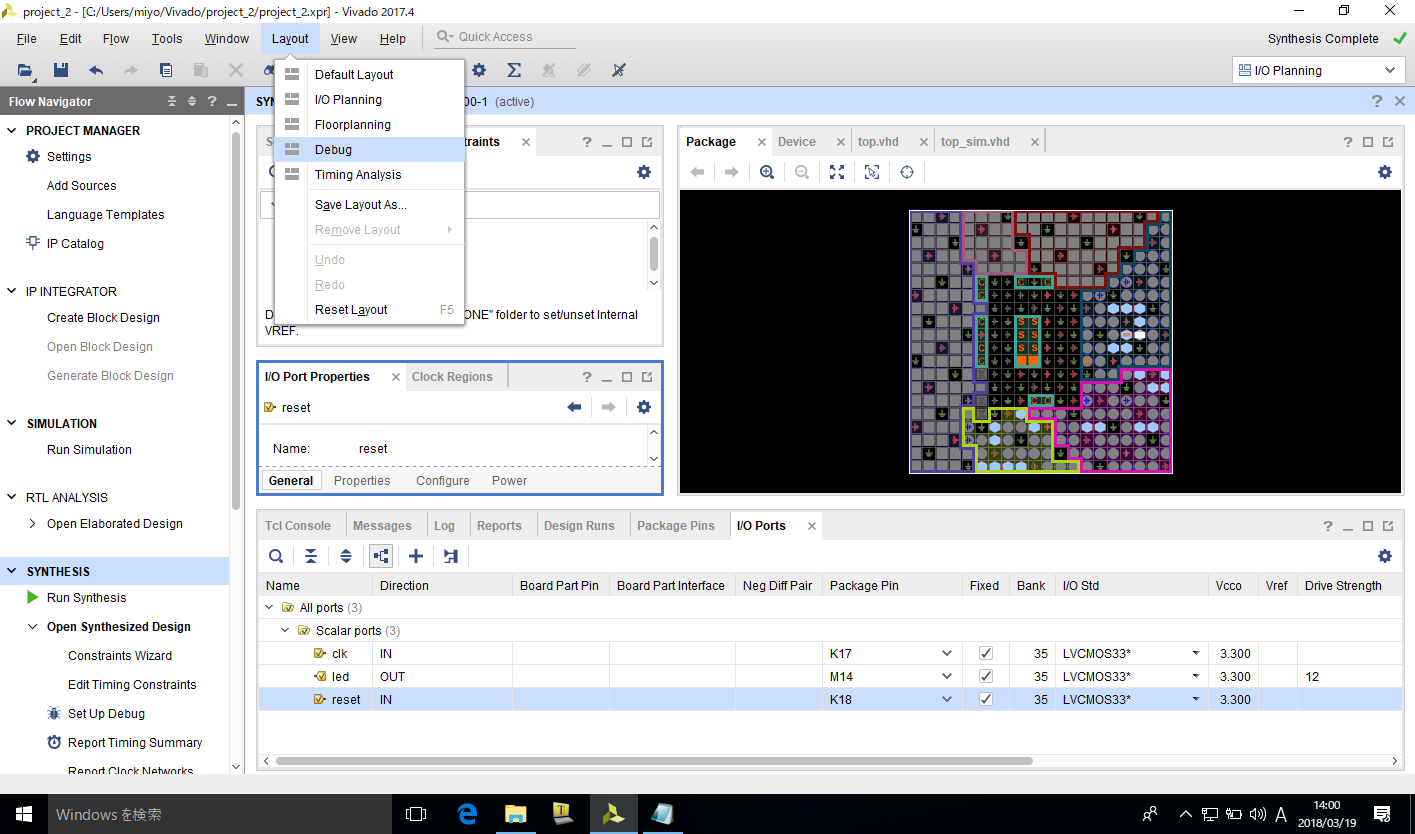
\includegraphics[width=.8\textwidth]{chapter05_figures/VirtualBox_Windows10_19_03_2018_14_00_09.png}
  \end{center}
  \caption{LayoutメニューのDebugをクリックしてデバッグビューに変更する}
 \end{figure}

 \begin{figure}[H]
  \begin{center}
   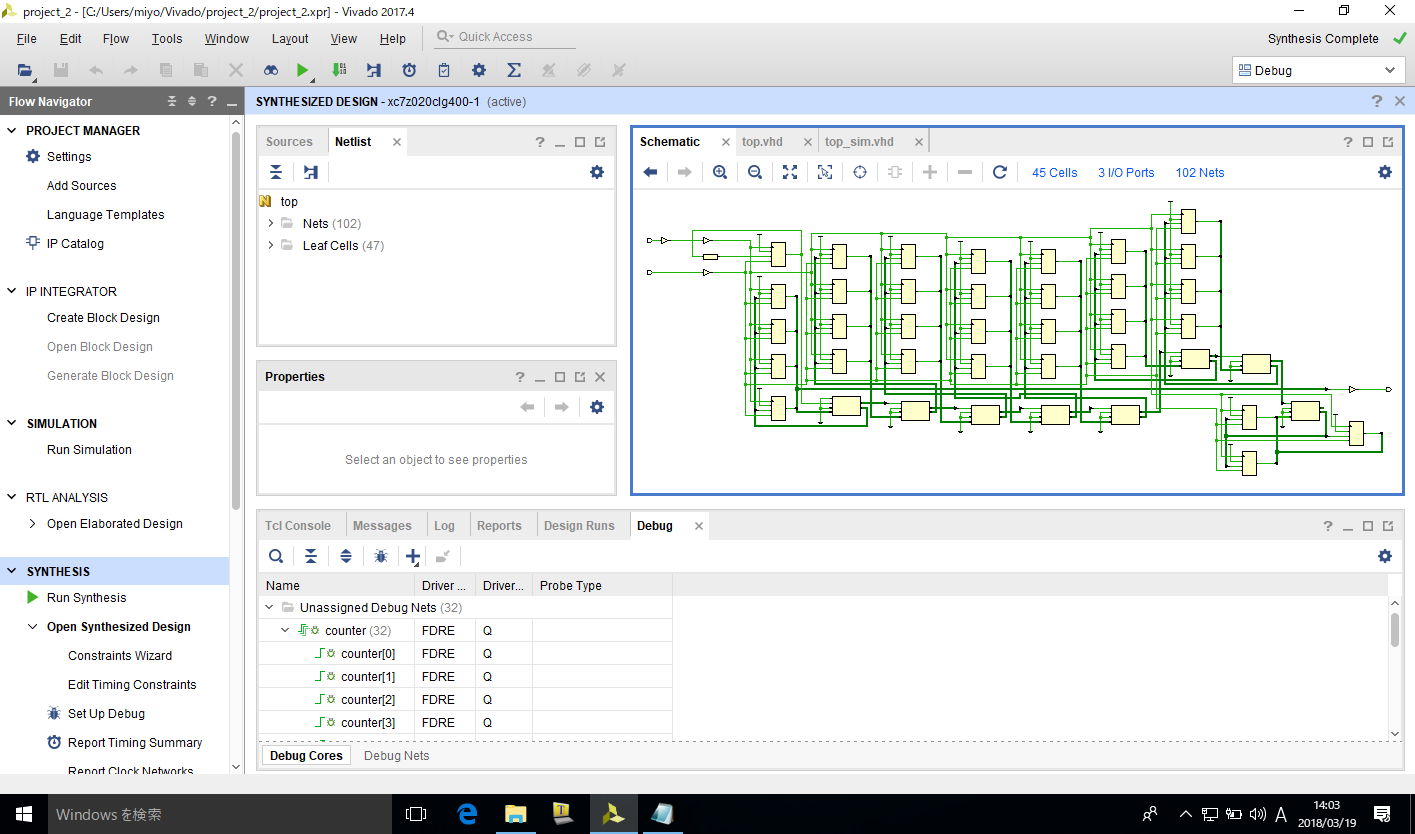
\includegraphics[width=.8\textwidth]{chapter05_figures/VirtualBox_Windows10_19_03_2018_14_03_37.png}
  \end{center}
  \caption{ILA設定用の画面 \label{fig:debug_mode_view}}
 \end{figure}

 \begin{figure}[H]
  \begin{center}
   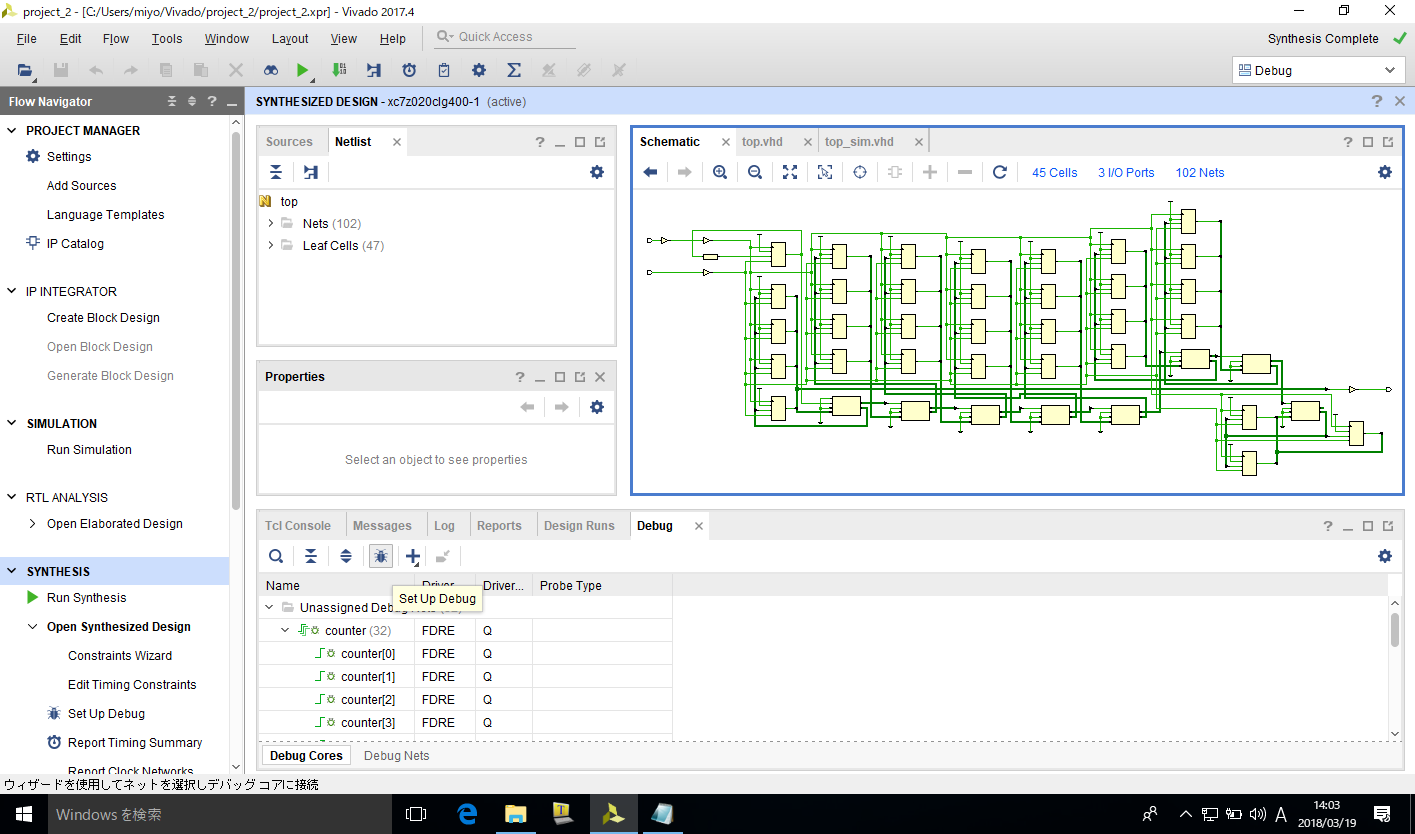
\includegraphics[width=.8\textwidth]{chapter05_figures/VirtualBox_Windows10_19_03_2018_14_03_43.png}
  \end{center}
  \caption{下にある虫みたいなアイコンをクリックしてILA設定用のウィザードを開く}
 \end{figure}

 \begin{figure}[H]
  \begin{center}
   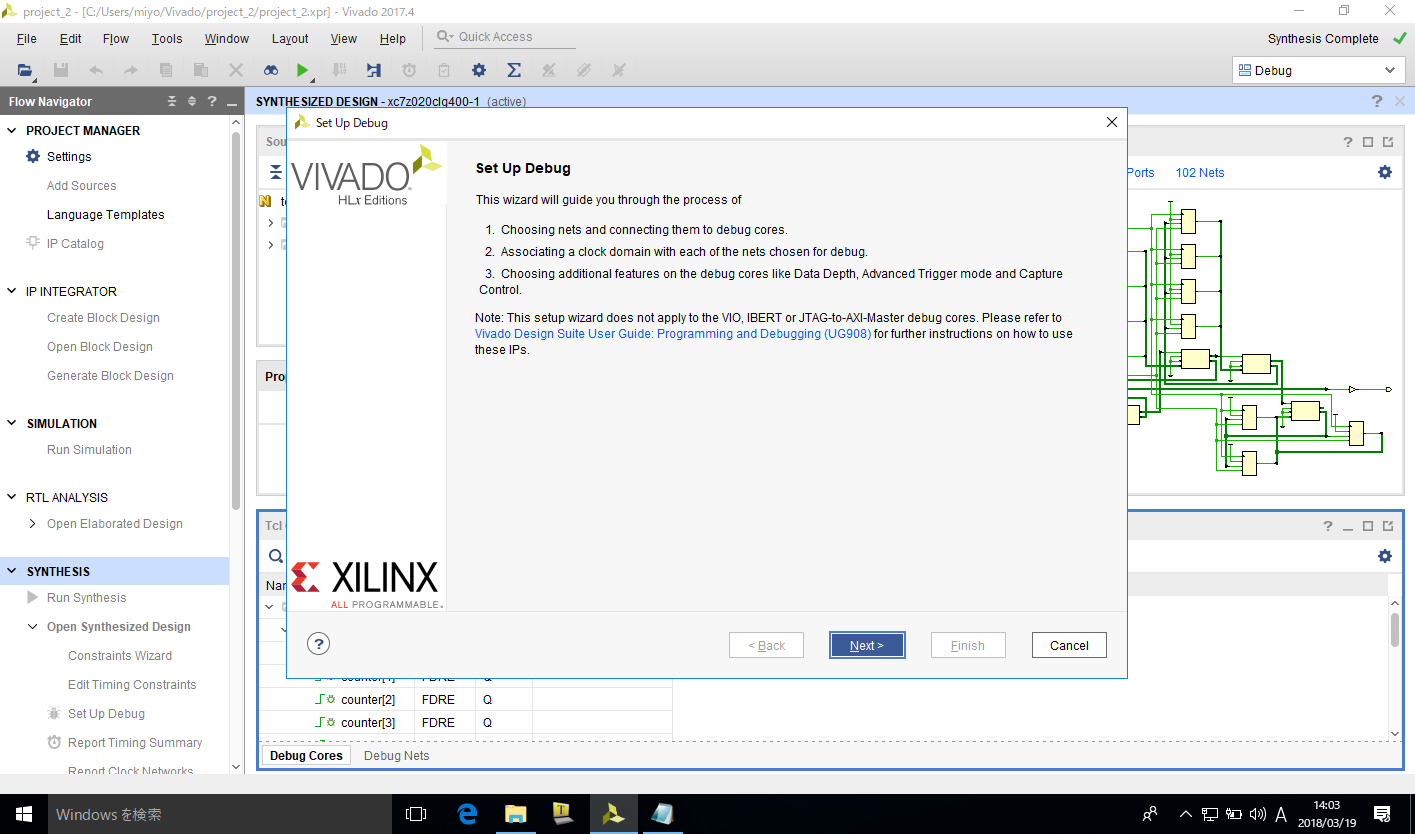
\includegraphics[width=.8\textwidth]{chapter05_figures/VirtualBox_Windows10_19_03_2018_14_03_58.png}
  \end{center}
  \caption{ILA設定用ウィザードの開始}
 \end{figure}

 \begin{figure}[H]
  \begin{center}
   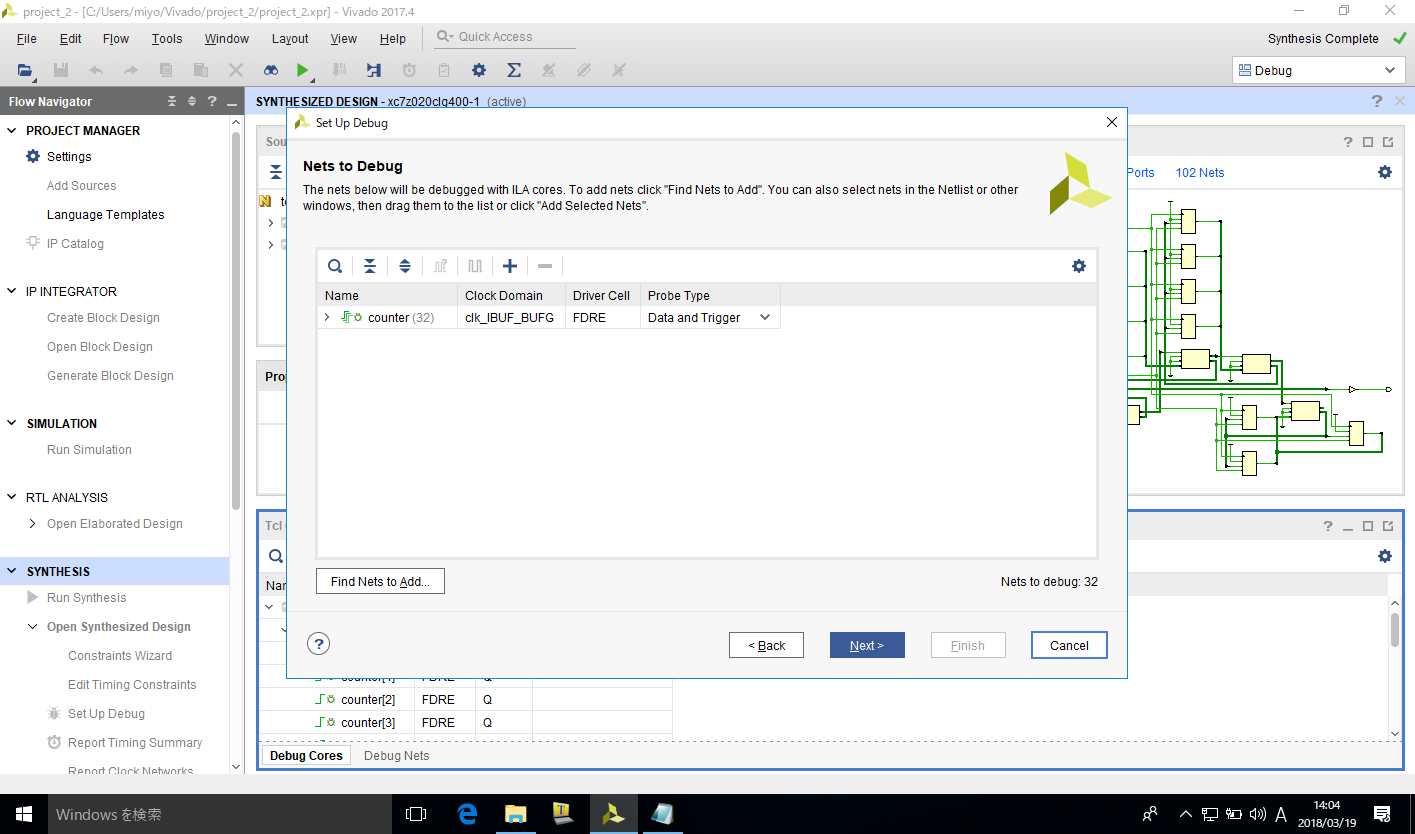
\includegraphics[width=.8\textwidth]{chapter05_figures/VirtualBox_Windows10_19_03_2018_14_04_03.png}
  \end{center}
  \caption{mark\_debugを付与したcounterがリストに追加されているので,そのままNextですすむ.ここで新たにILAによる観測対象を追加したい場合には+アイコンをクリックすると信号を選ぶことができる.逆にリストにある信号を対象から取り除きたい場合には,取り除きたい信号を選択して-をクリックする}
 \end{figure}

 \begin{figure}[H]
  \begin{center}
   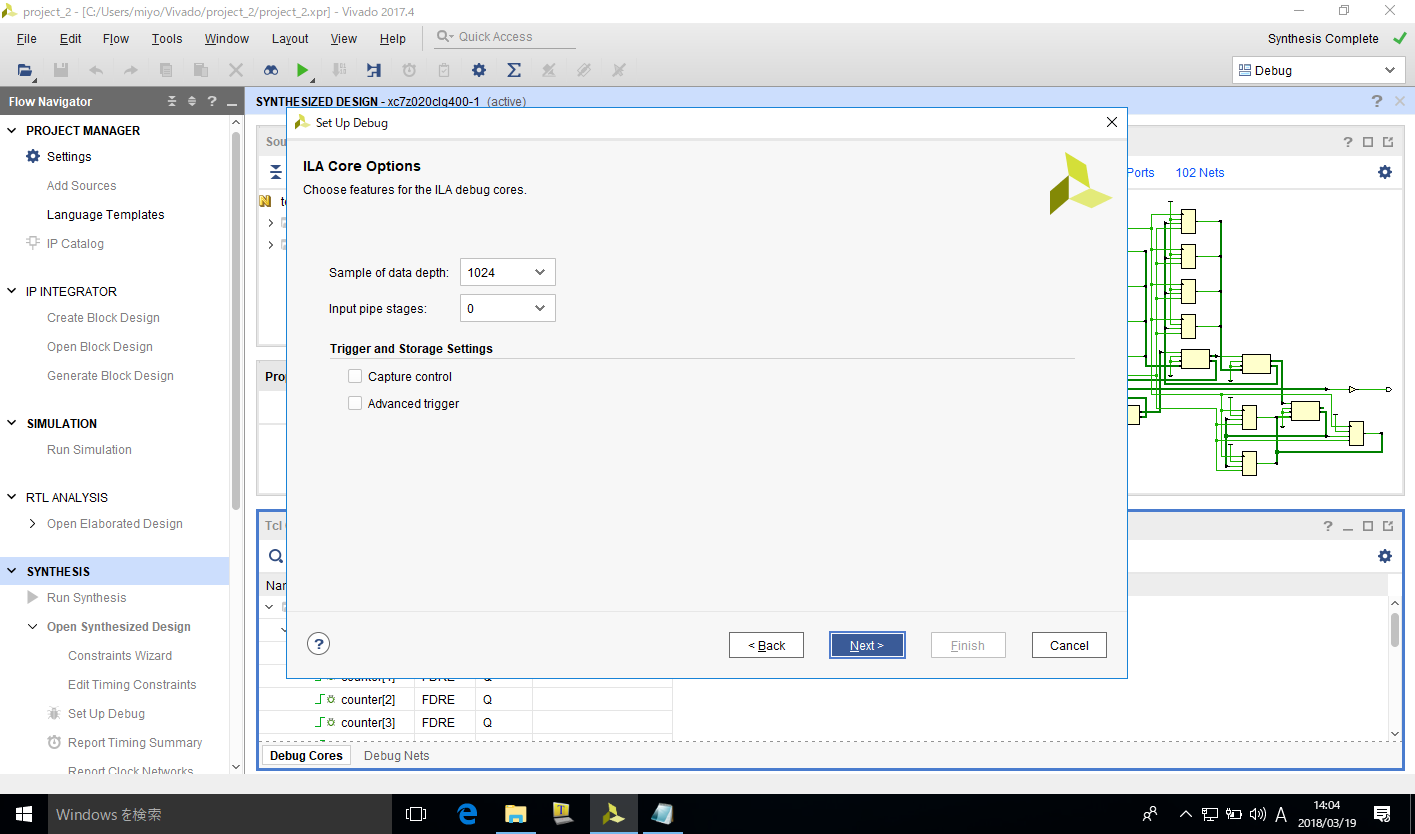
\includegraphics[width=.8\textwidth]{chapter05_figures/VirtualBox_Windows10_19_03_2018_14_04_08.png}
  \end{center}
  \caption{ILAで取得するデータ数の設定など.今回はそのままにしてNextですすむ}
 \end{figure}

 \begin{figure}[H]
  \begin{center}
   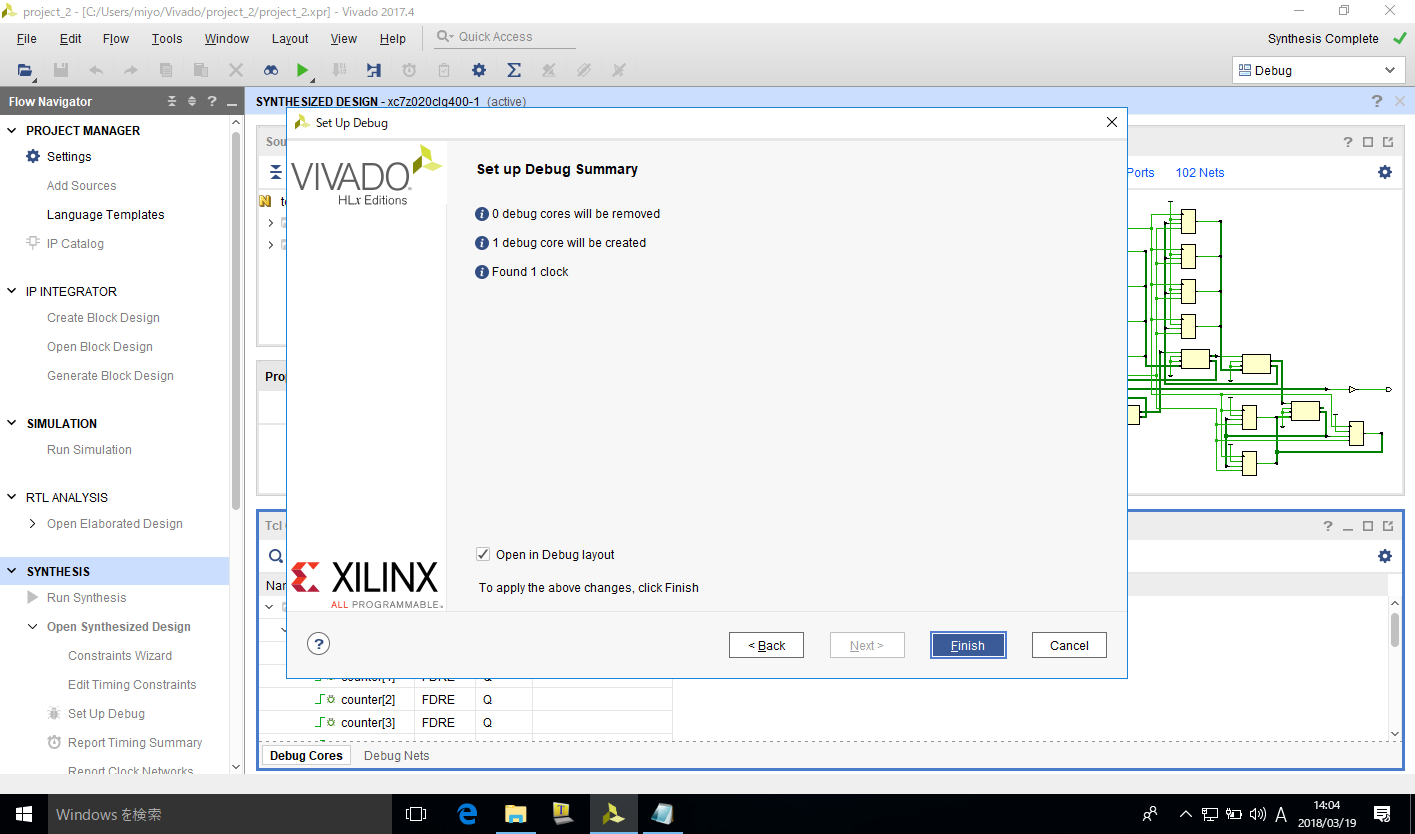
\includegraphics[width=.8\textwidth]{chapter05_figures/VirtualBox_Windows10_19_03_2018_14_04_13.png}
  \end{center}
  \caption{サマリの表示.Finishで完了}
 \end{figure}

 \begin{figure}[H]
  \begin{center}
   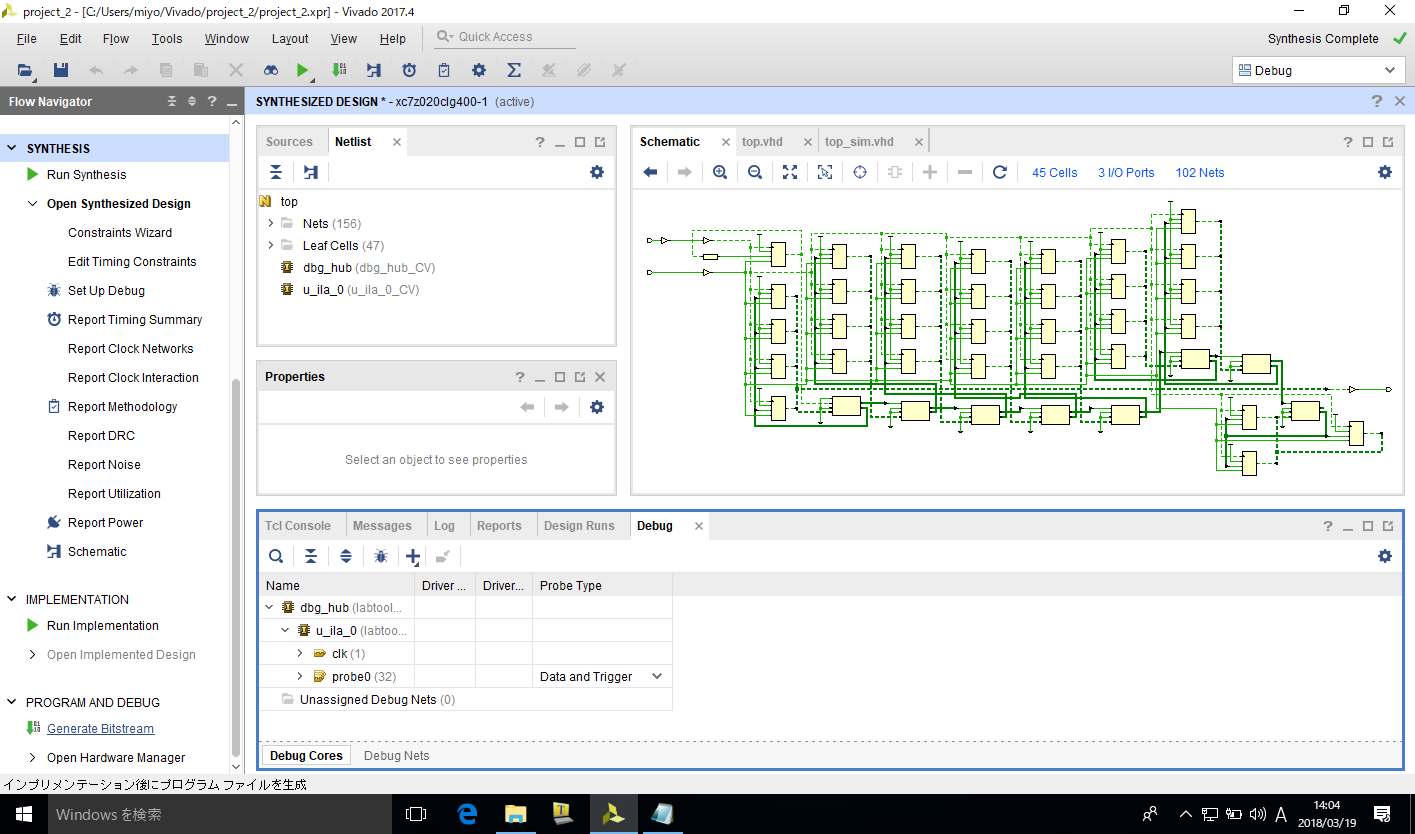
\includegraphics[width=.8\textwidth]{chapter05_figures/VirtualBox_Windows10_19_03_2018_14_04_28.png}
  \end{center}
  \caption{ウィザードが閉じてILAの設定は完了.ILAが追加できていることがわかる.あとは,Generate Bitstreamでビットファイルを作成すればよい.}
 \end{figure}

 \begin{figure}[H]
  \begin{center}
   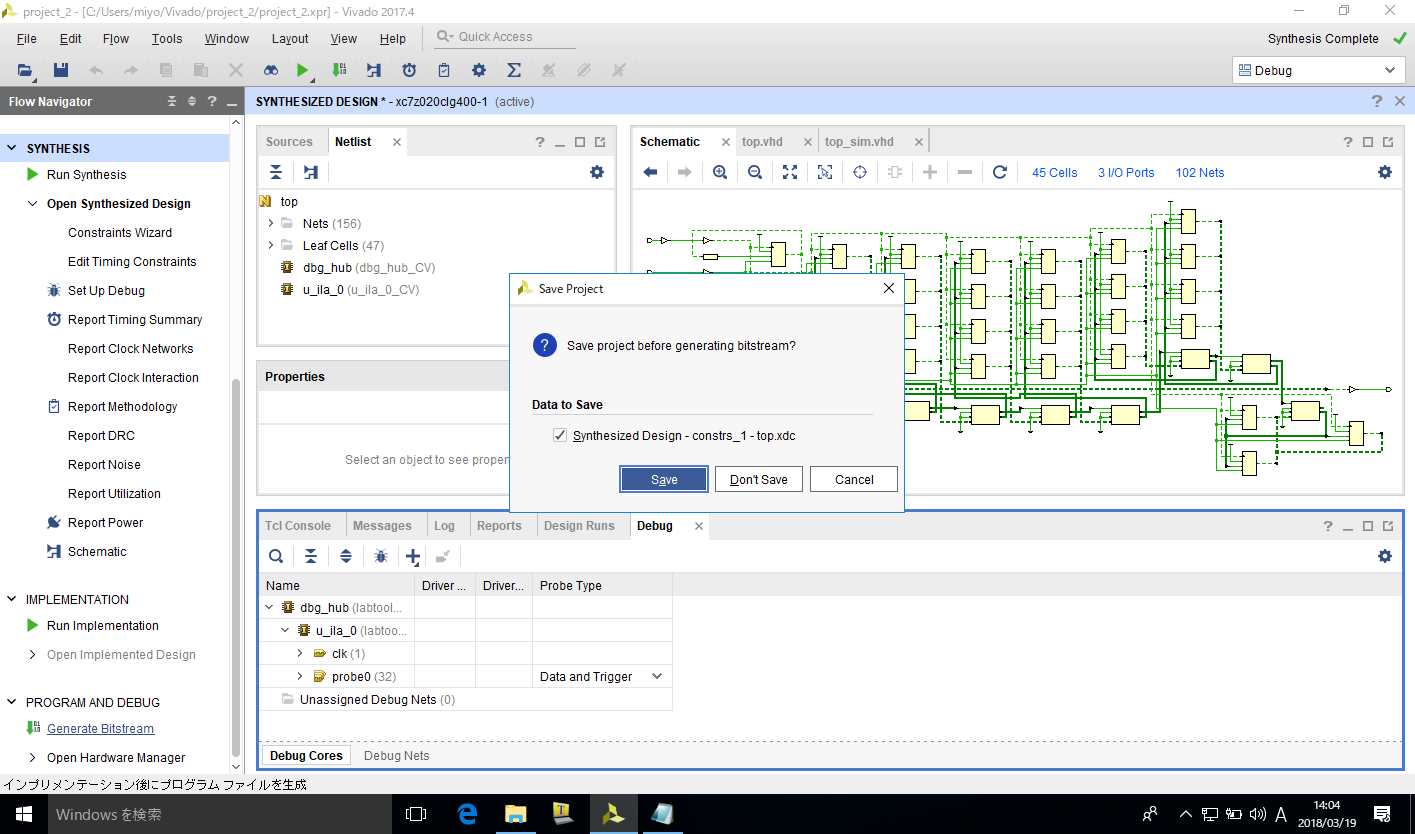
\includegraphics[width=.8\textwidth]{chapter05_figures/VirtualBox_Windows10_19_03_2018_14_04_33.png}
  \end{center}
  \caption{ILAの設定情報をxdcファイルに保存してよいかの確認.Yesで次のステップにすすむ.}
 \end{figure}

 \begin{figure}[H]
  \begin{center}
   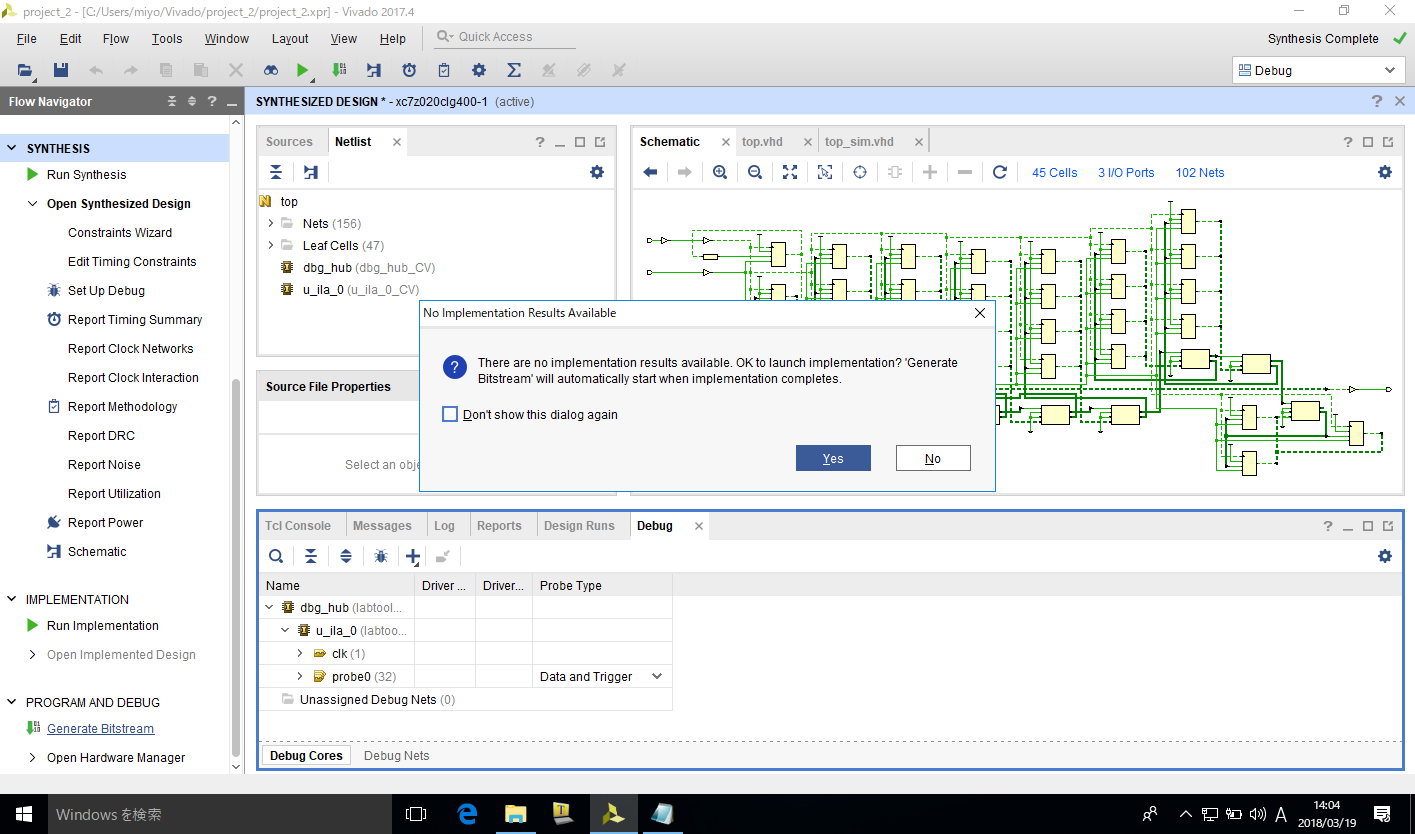
\includegraphics[width=.8\textwidth]{chapter05_figures/VirtualBox_Windows10_19_03_2018_14_04_44.png}
  \end{center}
  \caption{Generate bitstreamの前に依存する他のタスクを実行します,という確認ダイアログ.Yesで次のステップへ}
 \end{figure}

 \begin{figure}[H]
  \begin{center}
   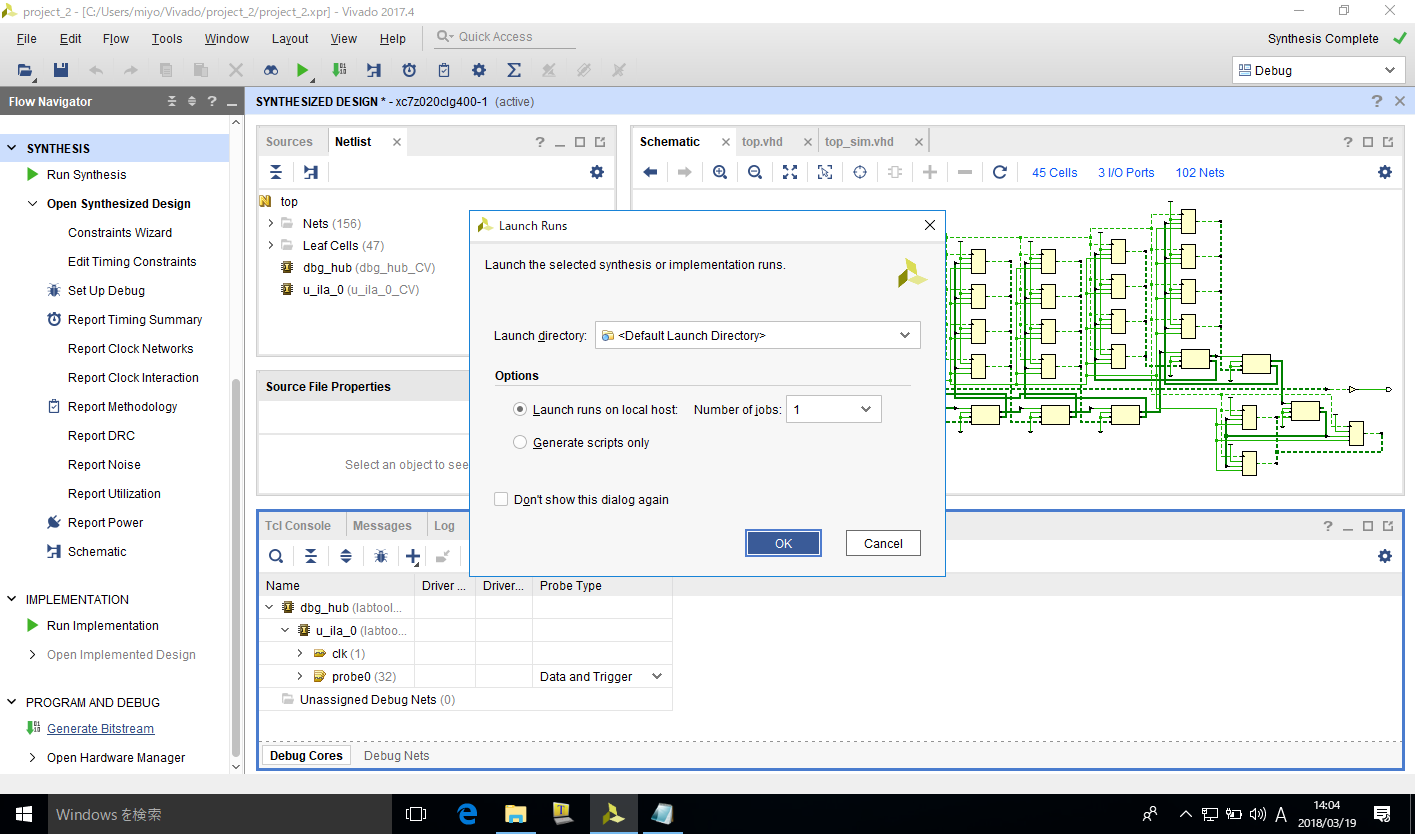
\includegraphics[width=.8\textwidth]{chapter05_figures/VirtualBox_Windows10_19_03_2018_14_04_49.png}
  \end{center}
  \caption{合成と配置配線の開始}
 \end{figure}

 \begin{figure}[H]
  \begin{center}
   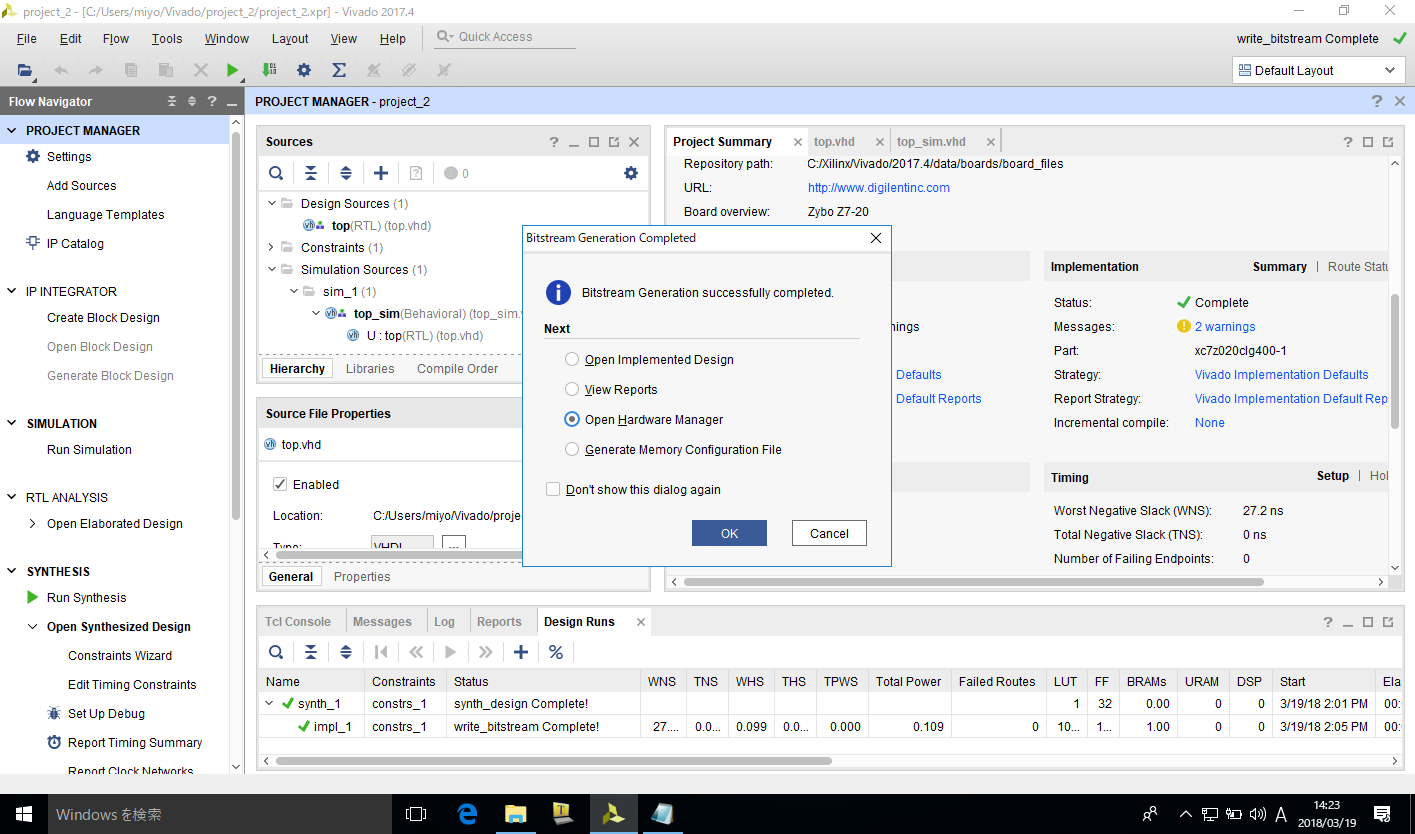
\includegraphics[width=.8\textwidth]{chapter05_figures/VirtualBox_Windows10_19_03_2018_14_23_17.png}
  \end{center}
  \caption{無事に合成と配置配線が終了しビットファイルができあがったところ.Open Hardware Managerを選択してOKをクリックすることで,ハードウェアマネージャの起動の手間を省くことができる}
 \end{figure}

 \begin{figure}[H]
  \begin{center}
   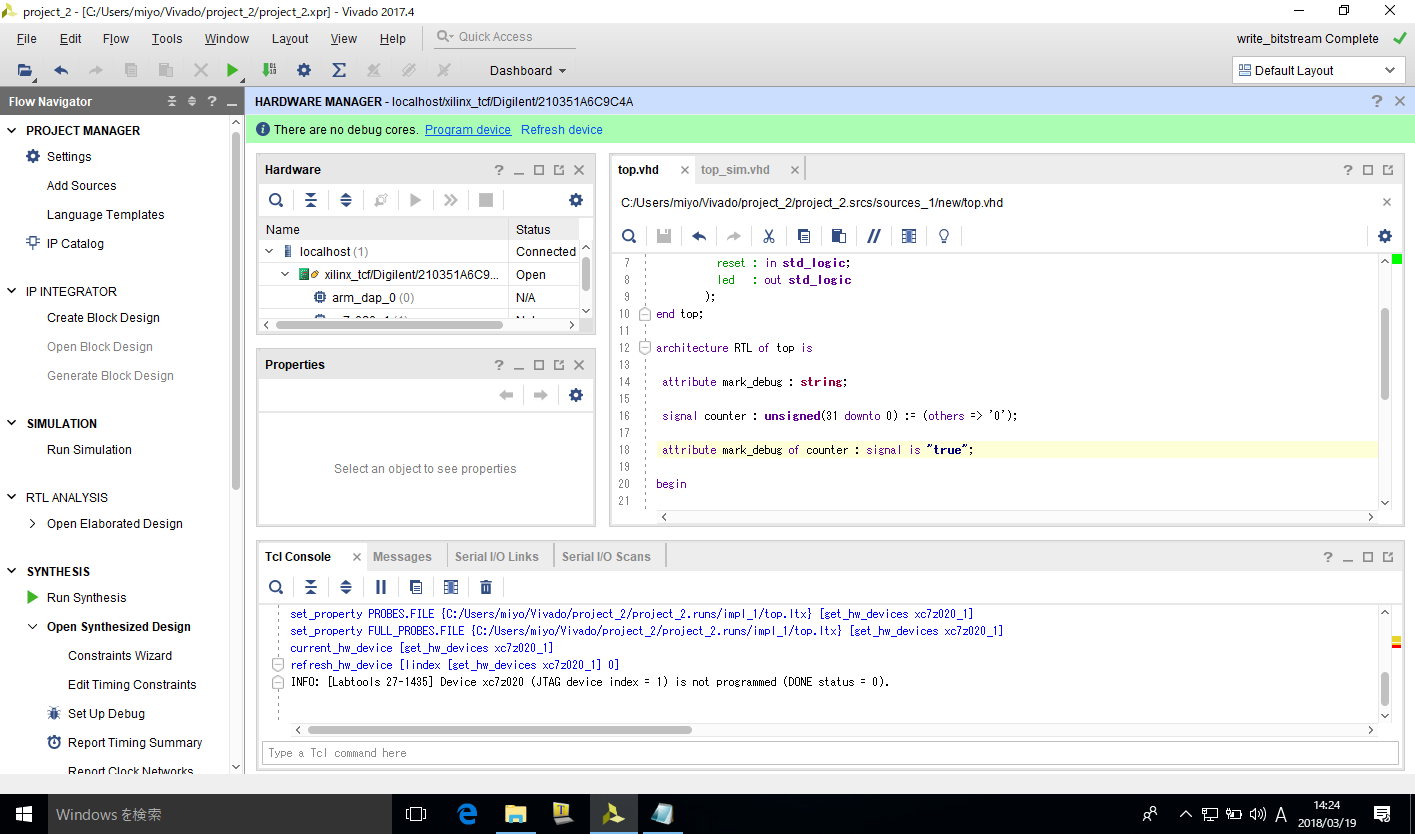
\includegraphics[width=.8\textwidth]{chapter05_figures/VirtualBox_Windows10_19_03_2018_14_23_59.png}
  \end{center}
  \caption{FPGAとパソコンをUSBケーブルで接続してAuto connectで認識させた後,Program Deviceをクリック}
 \end{figure}

 \begin{figure}[H]
  \begin{center}
   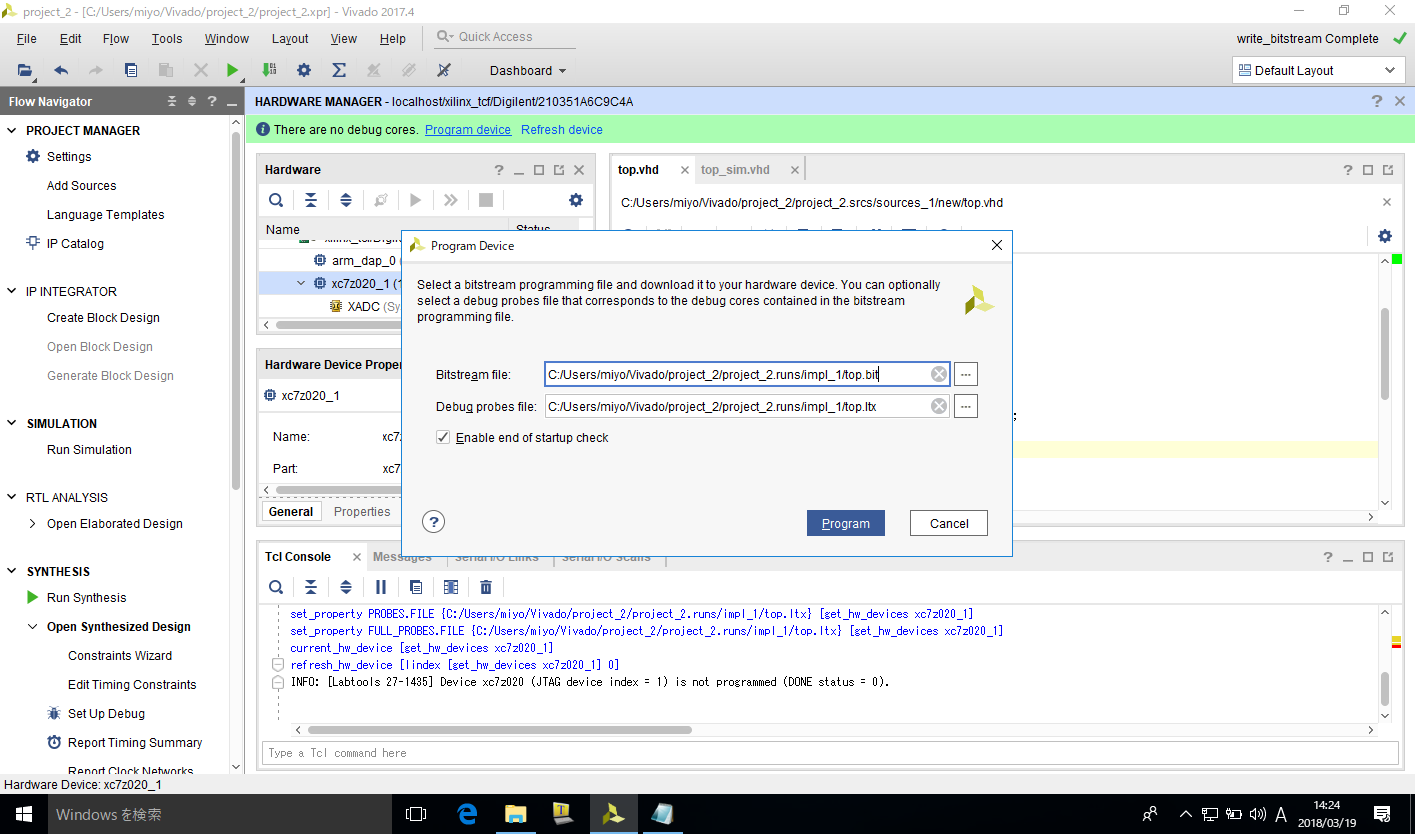
\includegraphics[width=.8\textwidth]{chapter05_figures/VirtualBox_Windows10_19_03_2018_14_24_06.png}
  \end{center}
  \caption{bitファイルはFPGAに,ILAのパソコン側の定義ファイルであるilxはVivadoに読み込ませる.}
 \end{figure}

 \begin{figure}[H]
  \begin{center}
   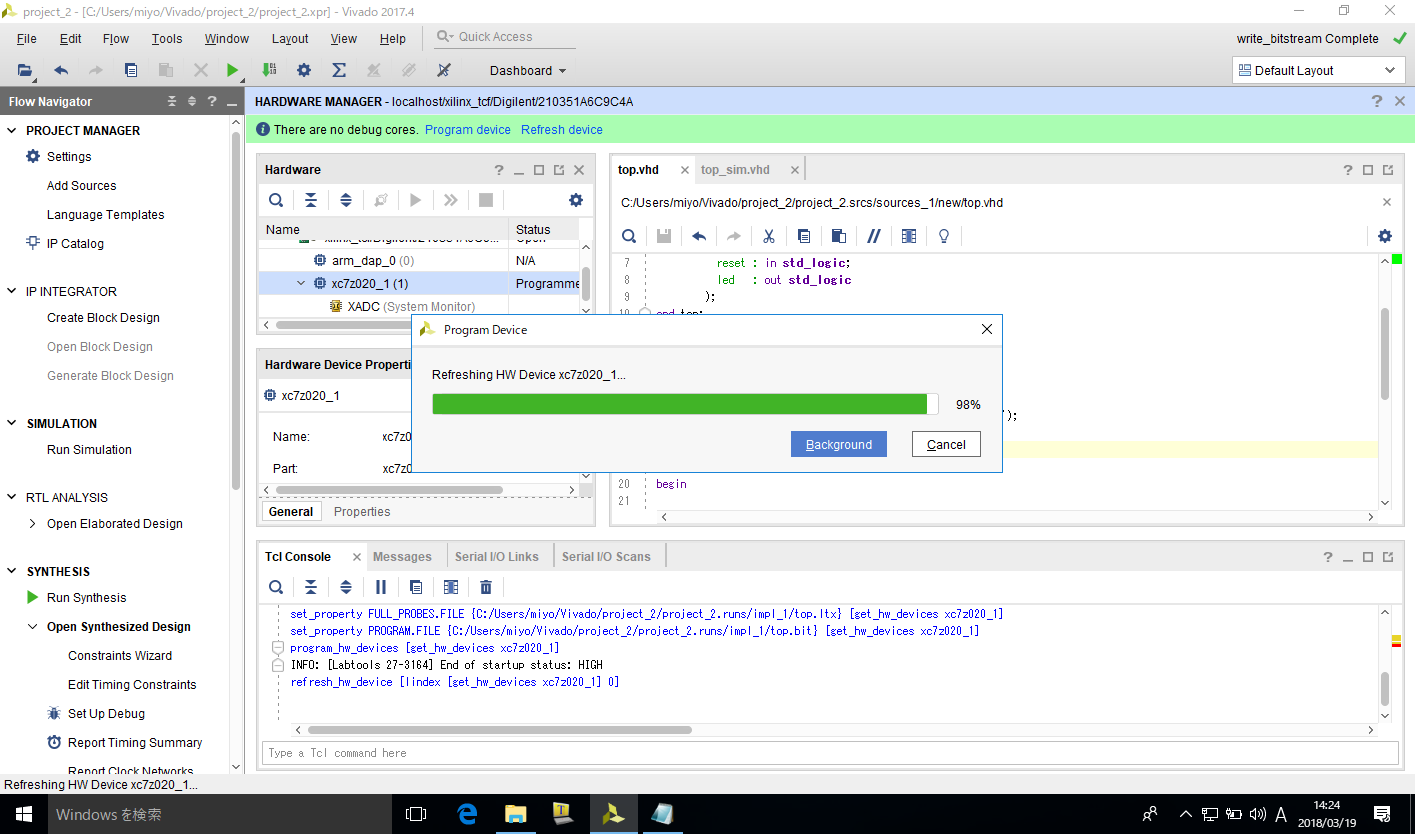
\includegraphics[width=.8\textwidth]{chapter05_figures/VirtualBox_Windows10_19_03_2018_14_24_16.png}
  \end{center}
  \caption{書き込み中}
 \end{figure}

 \begin{figure}[H]
  \begin{center}
   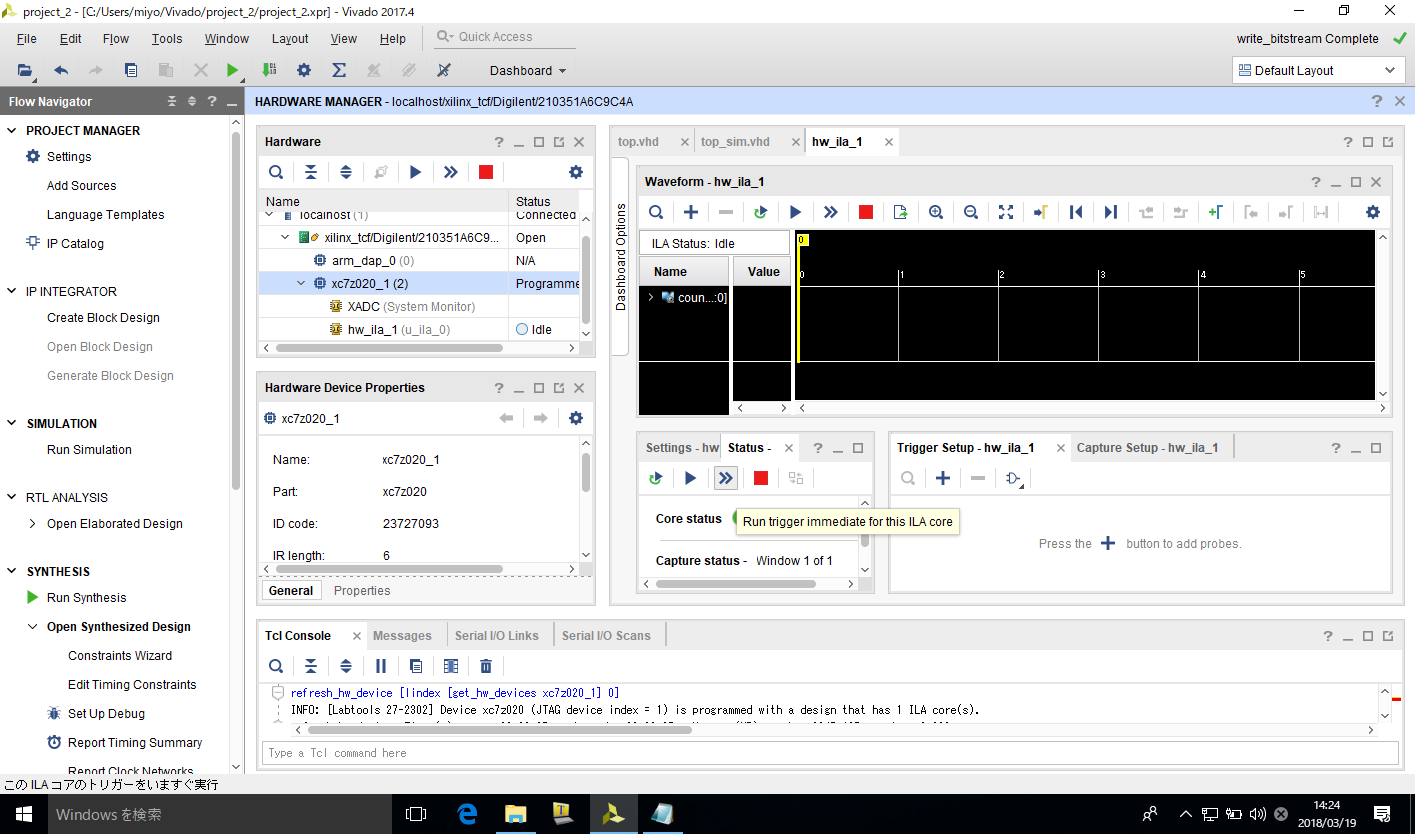
\includegraphics[width=.8\textwidth]{chapter05_figures/VirtualBox_Windows10_19_03_2018_14_24_38.png}
  \end{center}
  \caption{FPGAへのダウンロードが終了した.また,ILAによる動作のモニタ画面が表示された}
 \end{figure}

 \begin{figure}[H]
  \begin{center}
   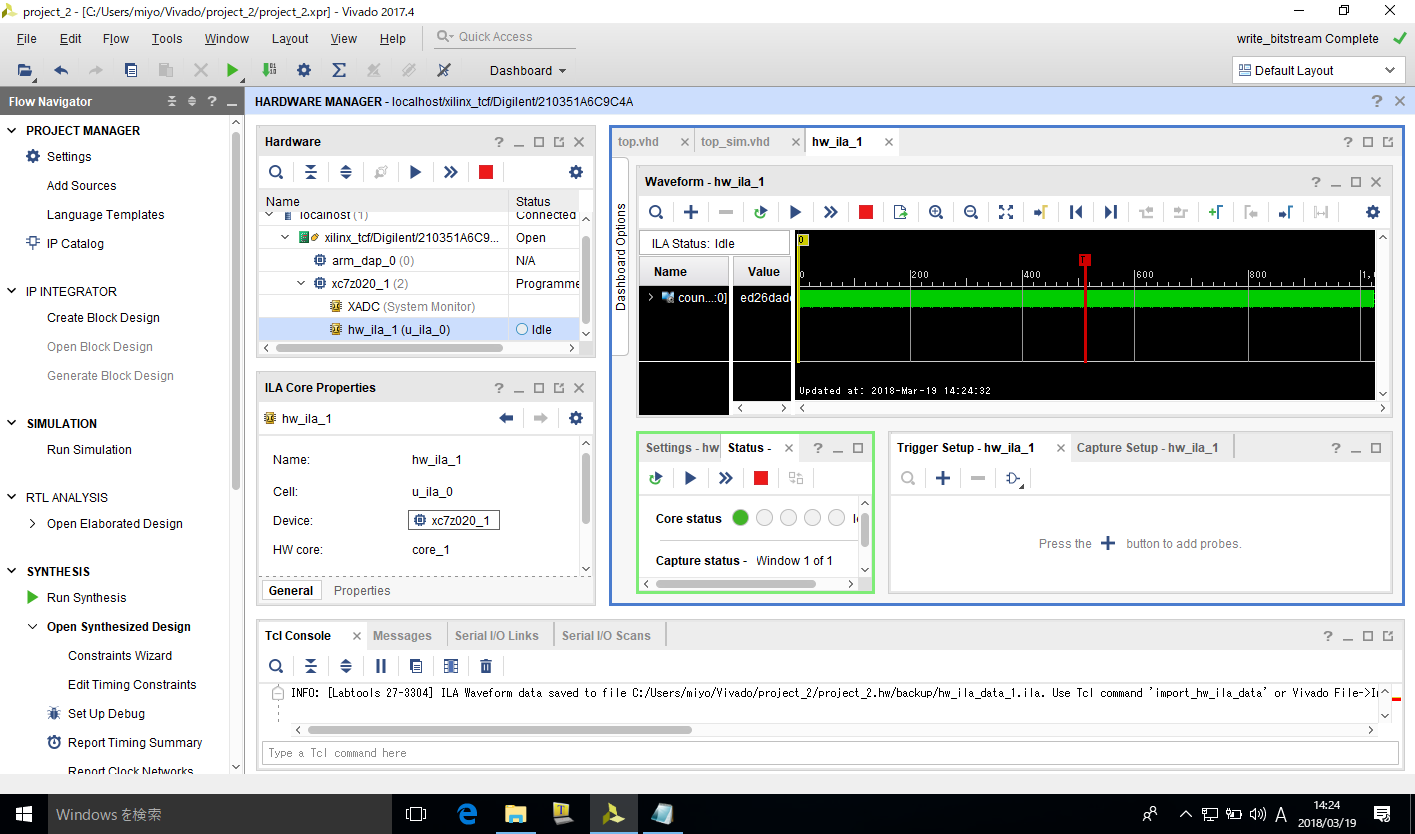
\includegraphics[width=.8\textwidth]{chapter05_figures/VirtualBox_Windows10_19_03_2018_14_24_53.png}
  \end{center}
  \caption{二重矢印のアイコンをクリックすると,その時点での値をキャプチャしてくれる}
 \end{figure}

 \begin{figure}[H]
  \begin{center}
   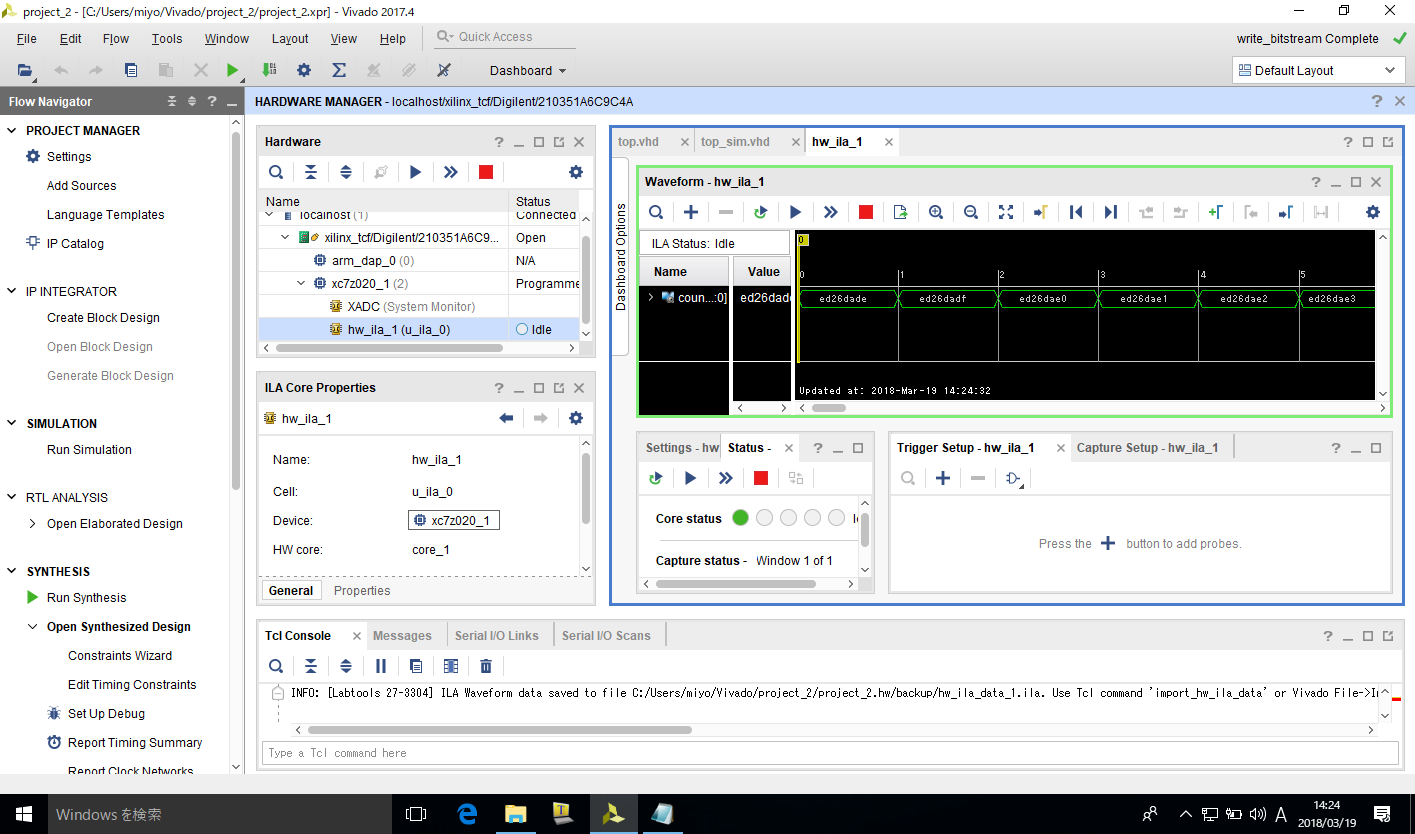
\includegraphics[width=.8\textwidth]{chapter05_figures/VirtualBox_Windows10_19_03_2018_14_25_07.png}
  \end{center}
  \caption{虫眼鏡アイコンで拡大すると,値が1ずつ増えていることが確認できる}
 \end{figure}

 \begin{figure}[H]
  \begin{center}
   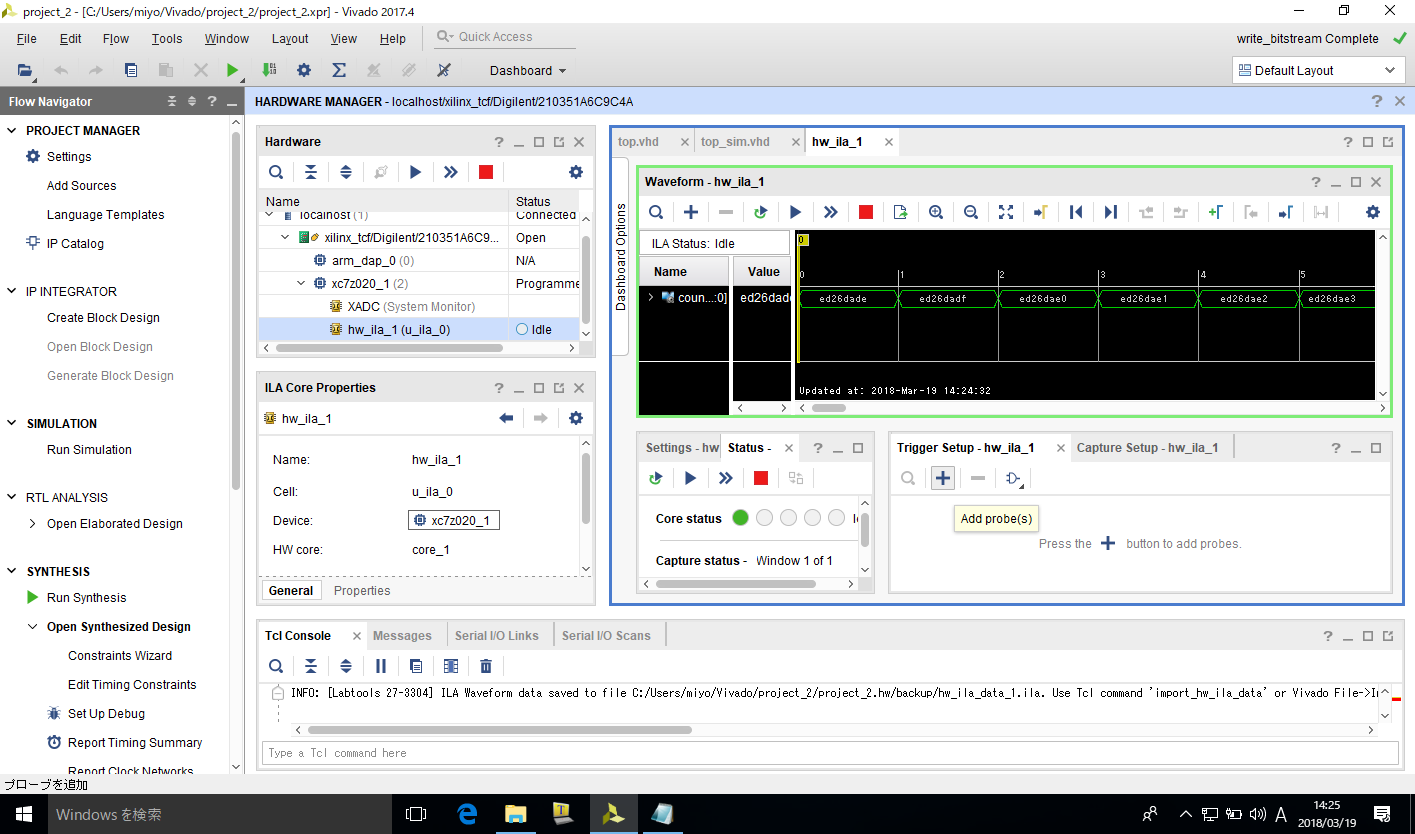
\includegraphics[width=.8\textwidth]{chapter05_figures/VirtualBox_Windows10_19_03_2018_14_25_21.png}
  \end{center}
  \caption{実機デバッガでは値をキャプチャする条件(トリガ条件)を指定する}
 \end{figure}

 \begin{figure}[H]
  \begin{center}
   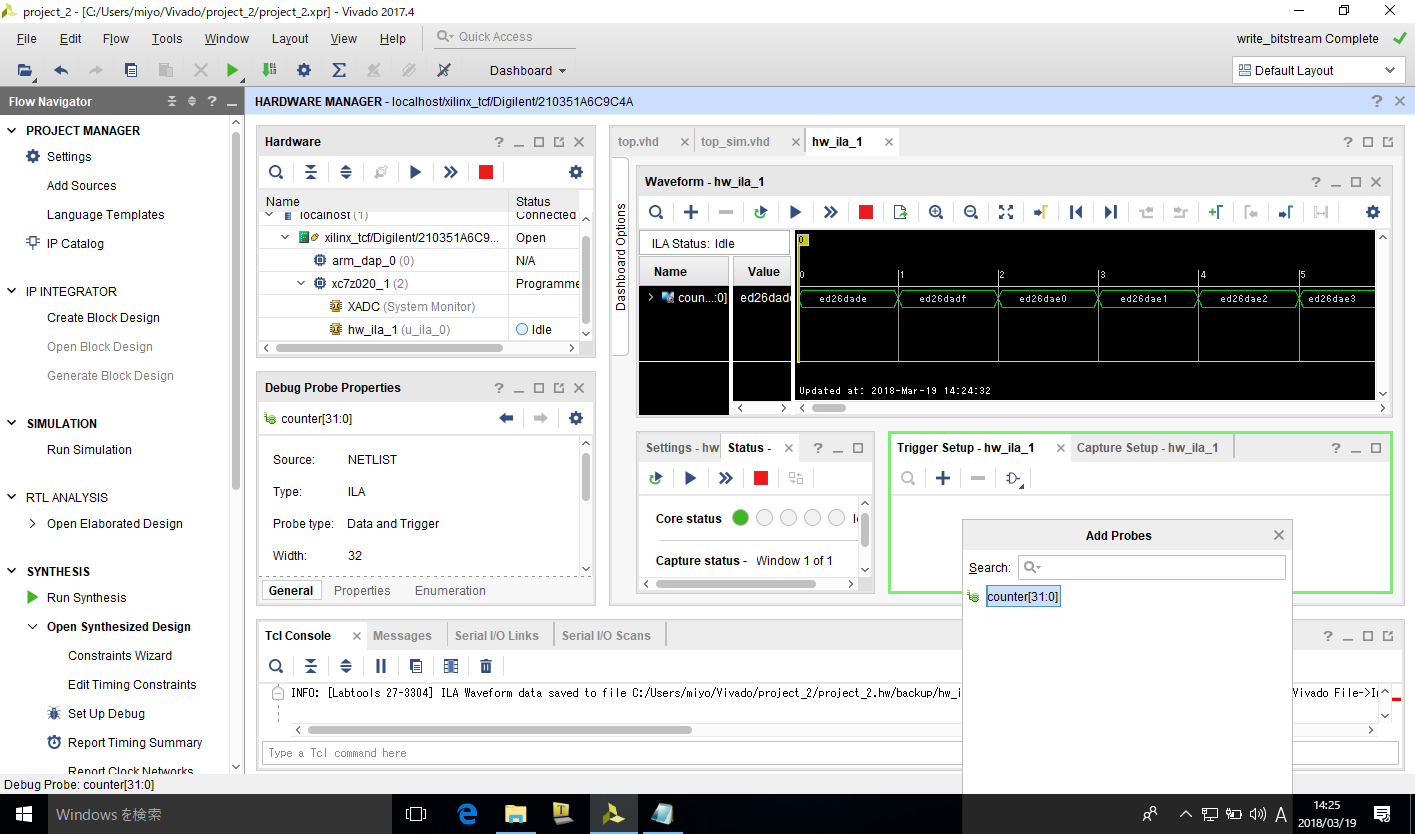
\includegraphics[width=.8\textwidth]{chapter05_figures/VirtualBox_Windows10_19_03_2018_14_25_27.png}
  \end{center}
  \caption{counterの値をトリガ条件に使用することとする}
 \end{figure}

 \begin{figure}[H]
  \begin{center}
   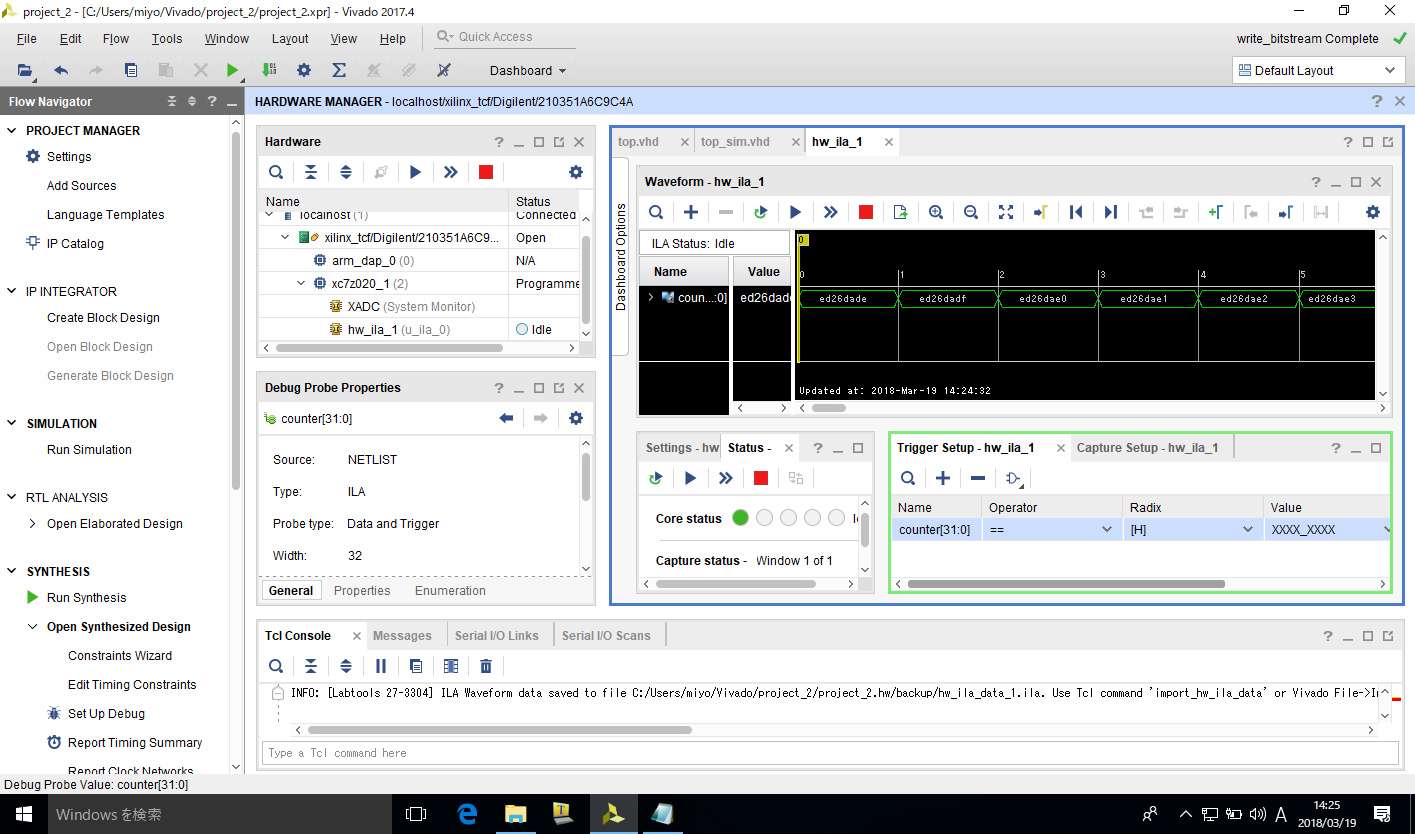
\includegraphics[width=.8\textwidth]{chapter05_figures/VirtualBox_Windows10_19_03_2018_14_25_34.png}
  \end{center}
  \caption{counterの値がトリガ条件として登録された}
 \end{figure}

 \begin{figure}[H]
  \begin{center}
   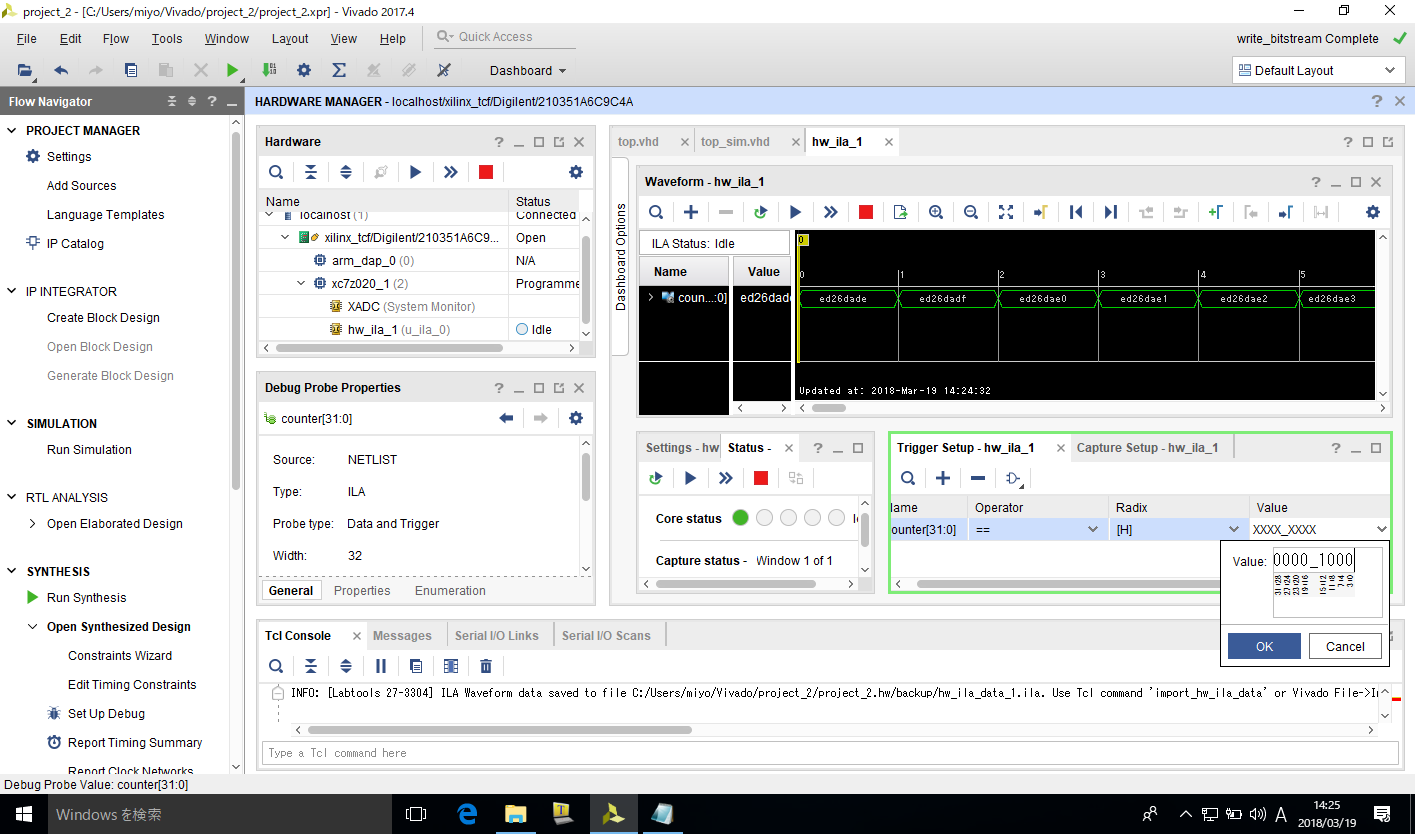
\includegraphics[width=.8\textwidth]{chapter05_figures/VirtualBox_Windows10_19_03_2018_14_25_50.png}
  \end{center}
  \caption{counterが00001000になった時点でキャプチャするように設定.トリガ値を指定したら三角アイコンでキャプチャを開始する}
 \end{figure}

 \begin{figure}[H]
  \begin{center}
   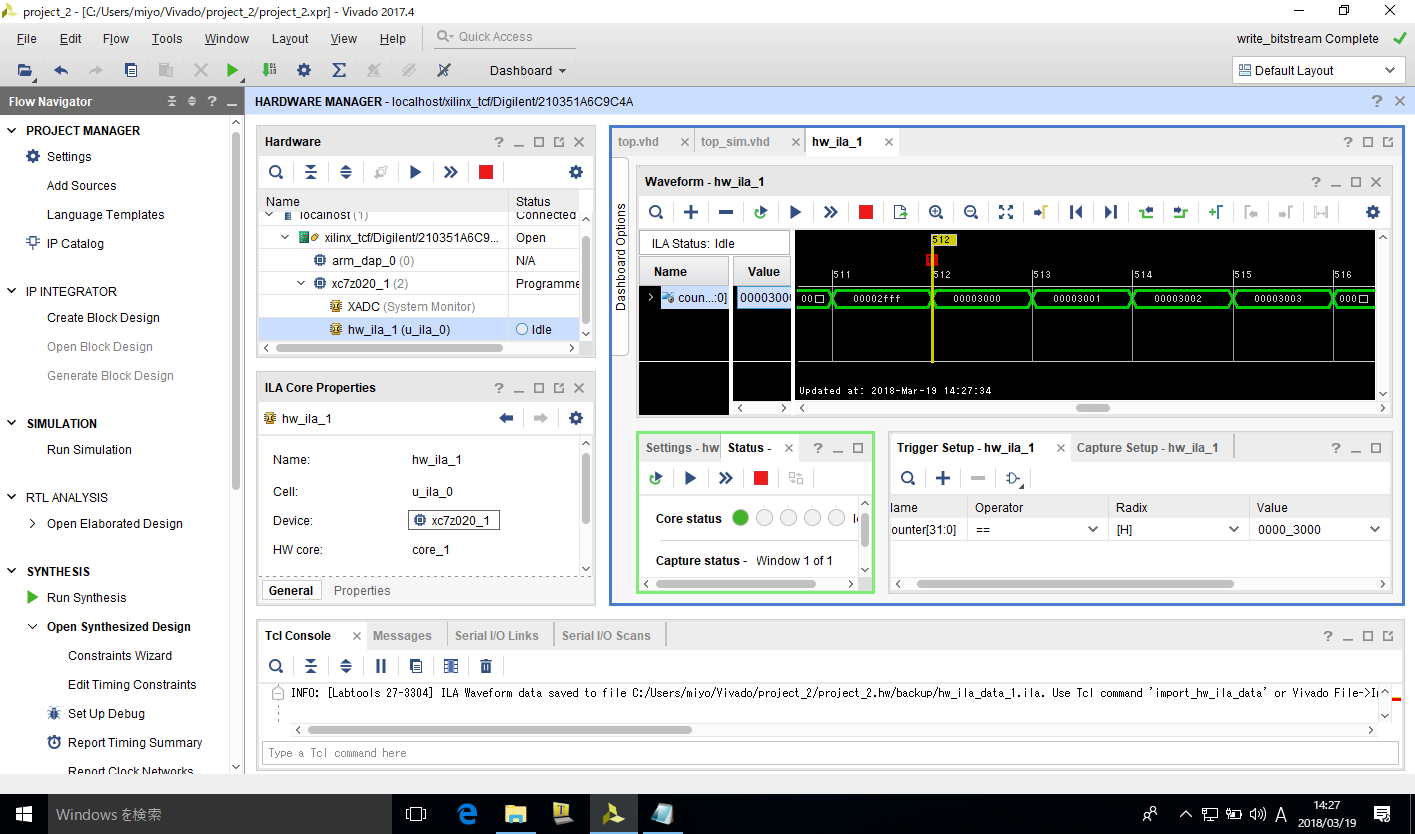
\includegraphics[width=.8\textwidth]{chapter05_figures/VirtualBox_Windows10_19_03_2018_14_27_49.png}
  \end{center}
  \caption{counterが00001000になった時点のデータをキャプチャすることができた}
 \end{figure}

 \begin{figure}[H]
  \begin{center}
   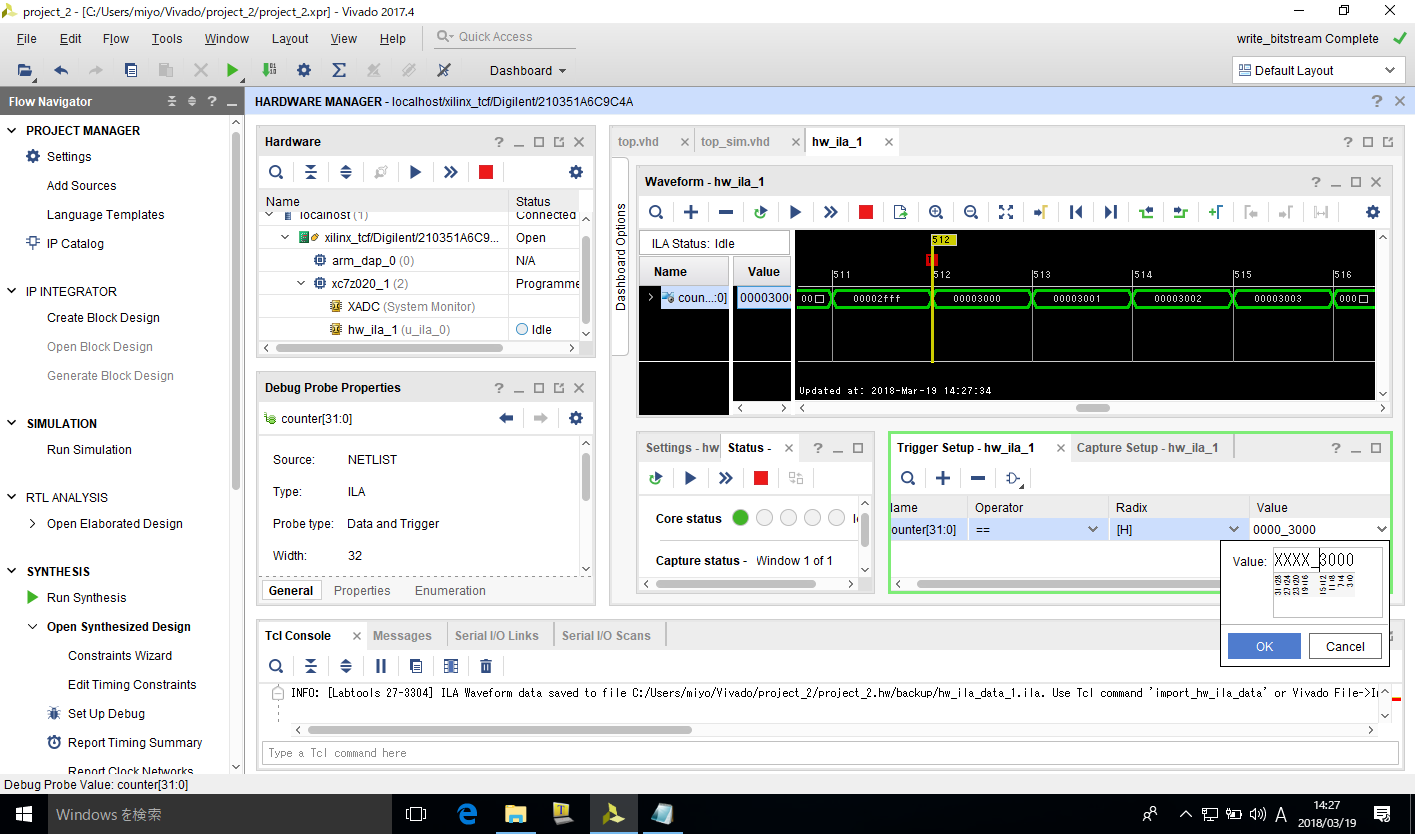
\includegraphics[width=.8\textwidth]{chapter05_figures/VirtualBox_Windows10_19_03_2018_14_28_03.png}
  \end{center}
  \caption{トリガにはドントケア(X)を指定することも可能.ここでは下位16bitが3000になるデータを取得するように指定してみる}
 \end{figure}

 \begin{figure}[H]
  \begin{center}
   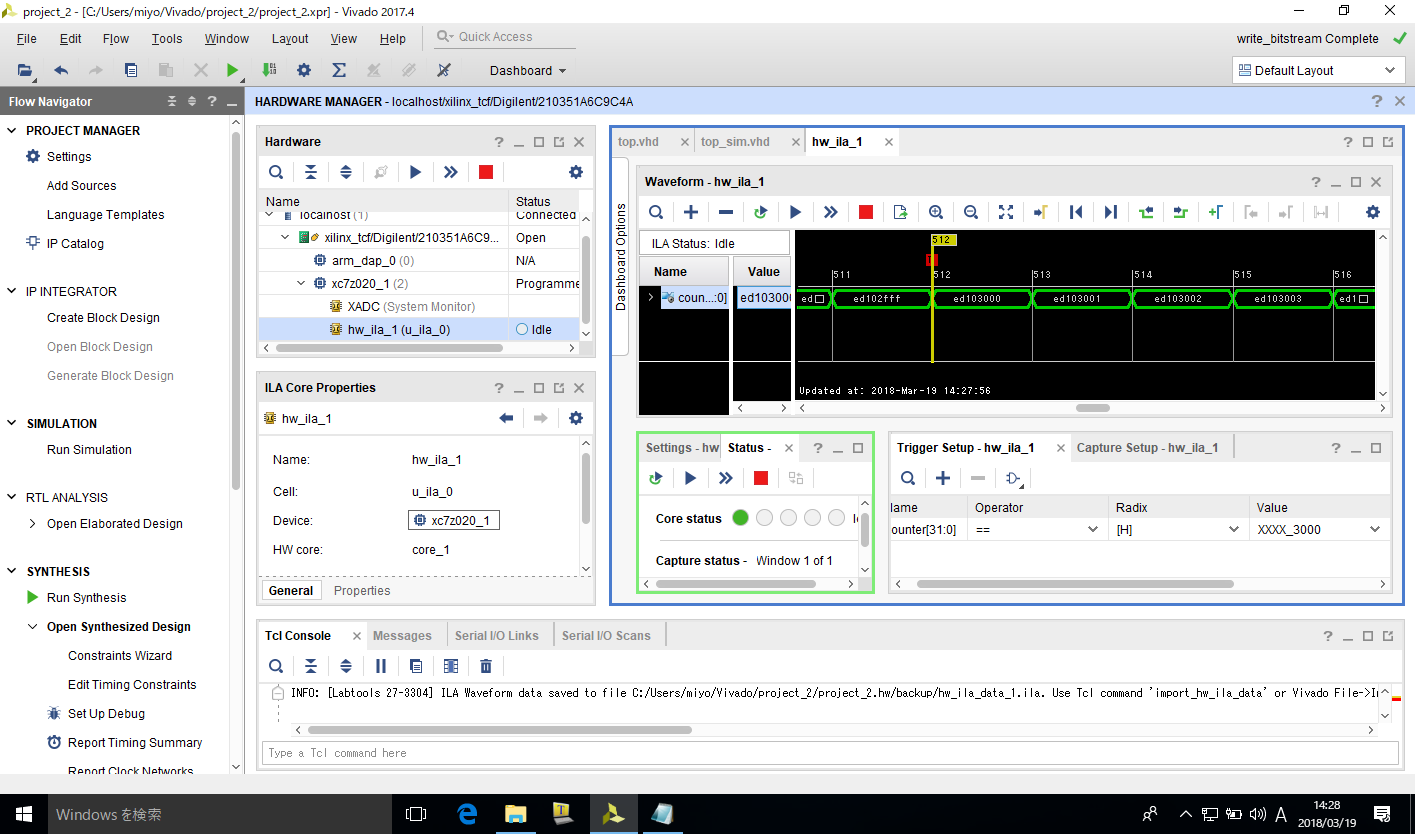
\includegraphics[width=.8\textwidth]{chapter05_figures/VirtualBox_Windows10_19_03_2018_14_28_15.png}
  \end{center}
  \caption{上位16bitは指定なく,下位16bitが3000の時点のデータがキャプチャできていることがわかる}
 \end{figure}

\subsection{ILA挿入すると回路は変わる}
重要な点ですが,ILAを挿入すると,挿入前とは異なるハードウェアになることを理解しておく必要があります.ILA向けのリソース使用量が増えるのはもちろん,観測対象の信号の接続関係も変化します.また観測のために残すべきレジスタの都合で最適化の結果もかわってきます.

たとえば,図\ref{fig:without_mark_debug}は,counterにmark\_debugアトリビュートを付与せずに合成した場合のデバッグビューです.3bit目をledに接続し,それ以上のbit数の値は利用さていないため,ばっさりと回路が小さくなっていることがわかります.

しかし,mark\_debugアトリビュートを付与して合成した場合には,もちろん最適化するわけにはいかないため,図\ref{fig:debug_mode_view}のように要/不要にかかわらず32bit分すべてのレジスタが回路として生成されています.

 \begin{figure}[H]
  \begin{center}
   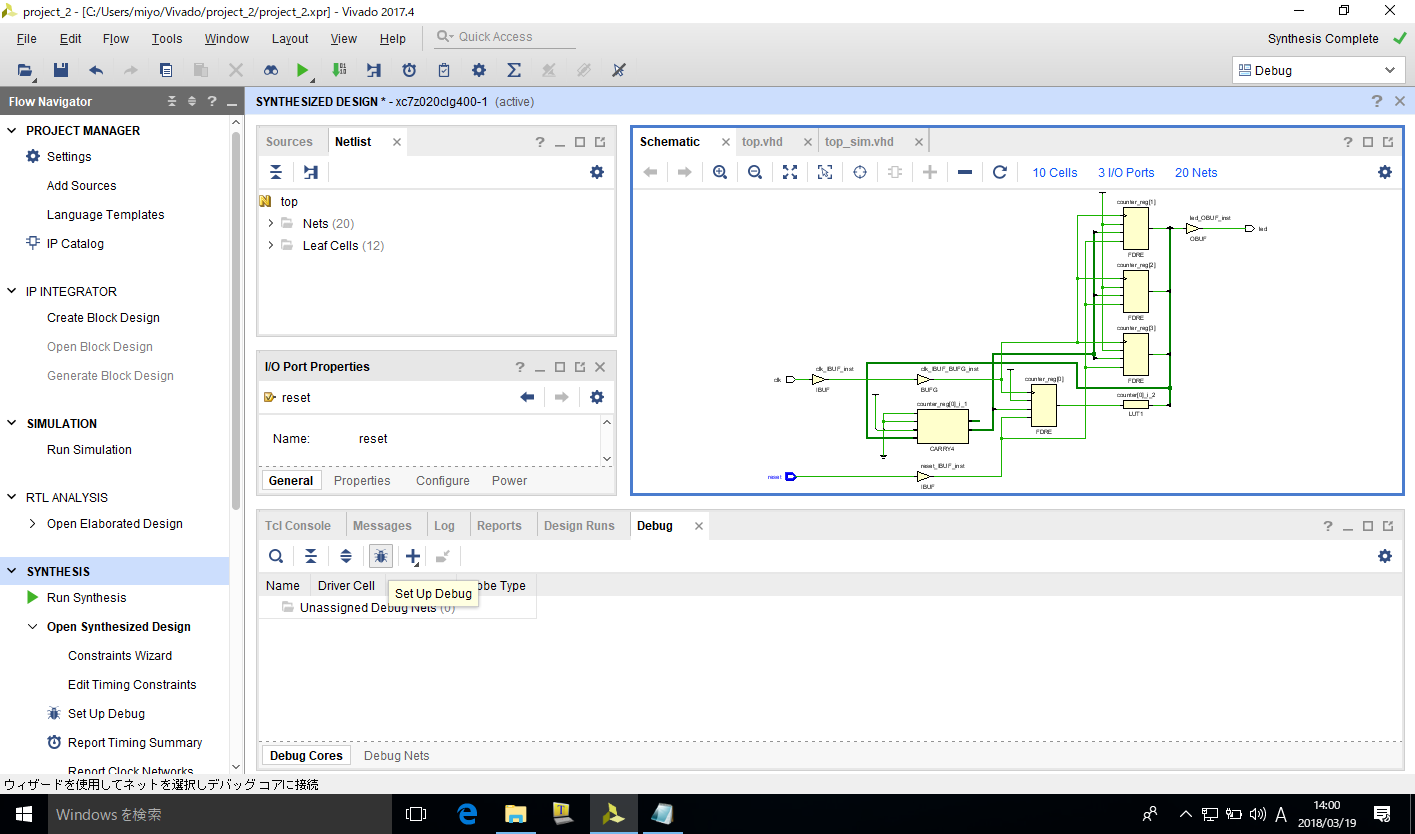
\includegraphics[width=.8\textwidth]{chapter05_figures/VirtualBox_Windows10_19_03_2018_14_00_24.png}
  \end{center}
  \caption{counterにmark\_debugがない場合 \label{fig:without_mark_debug}}
 \end{figure}


\section{基本実験の準備}
FPGAを使った実験をする前に,動作の様子を確認しながら実験できるように簡単なテンプレートモジュールを用意しておくことにします.
ここで作るのは,図\ref{fig:experiment_template}のように4bitの入力と4bitの出力ポートで構成されるモジュールです.
ZYBOのDIPスイッチSW0〜SW3を4bitの入力に,LED LD0〜LD3を4bitの出力にマッピングすることにします.

 \begin{figure}[H]
  \begin{center}
   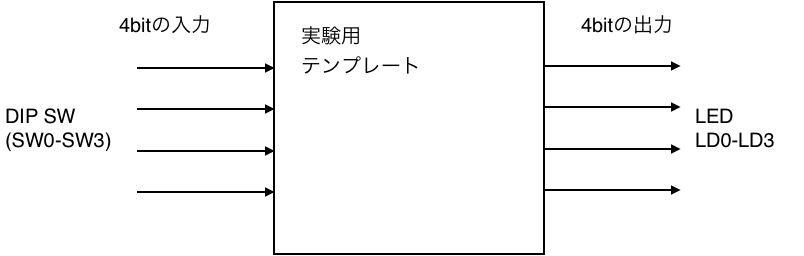
\includegraphics[width=.6\textwidth]{chapter05_figures/experiment_template.png}
  \end{center}  
  \caption{実験用の簡単なテンプレートモジュール \label{fig:experiment_template}}
 \end{figure}

次のような内容のVHDLファイルを用意します.

\begin{figure}[H]
\begin{quote}
\begin{Verbatim}[frame=single, numbers=left, baselinestretch=0.8]
library ieee;

use ieee.std_logic_1164.all;
use ieee.numeric_std.all;

entity top is
  port (
    CLK : in  std_logic;
    SW  : in  std_logic_vector(3 downto 0);
    LD  : out std_logic_vector(3 downto 0)
    );
end entity top;

architecture RTL of top is

  signal sw_d0 : std_logic_vector(3 downto 0);
  signal sw_d1 : std_logic_vector(3 downto 0);
  
begin

  LD <= sw_d1;
  
  process(CLK)
  begin
    if rising_edge(CLK) then
      sw_d0 <= SW;
      sw_d1 <= sw_d0;
    end if;
  end process;
  
end RTL;
\end{Verbatim}
\end{quote}
\end{figure}

ピン定義も用意しましょう.第3章で紹介したようにGUIで設定することもできますが,スクリプトファイルでピン定義を決めることもできます.実験に使用するZYBO Z7-20の全てのI/O定義は\url{https://github.com/Digilent/digilent-xdc/blob/master/Zybo-Z7-Master.xdc}にまとまっています.URL先の情報に基づいて,使用するピンの定義をまとめると次のようになります.top.xdcなどと,拡張子を.xdcとしてファイルに保存します.
\begin{figure}[H]
\begin{quote}
\begin{Verbatim}[frame=single, numbers=left, baselinestretch=0.8]
set_property -dict {PACKAGE_PIN K17 IOSTANDARD LVCMOS33 } [get_ports {CLK}];
create_clock -add -name clk_pin -period 8.00 -waveform {0 4} [get_ports {CLK}];

set_property -dict {PACKAGE_PIN G15 IOSTANDARD LVCMOS33} [get_ports {SW[0]}];
set_property -dict {PACKAGE_PIN P15 IOSTANDARD LVCMOS33} [get_ports {SW[1]}];
set_property -dict {PACKAGE_PIN W13 IOSTANDARD LVCMOS33} [get_ports {SW[2]}];
set_property -dict {PACKAGE_PIN T16 IOSTANDARD LVCMOS33} [get_ports {SW[3]}];

set_property -dict {PACKAGE_PIN M14 IOSTANDARD LVCMOS33} [get_ports {LD[0]}];
set_property -dict {PACKAGE_PIN M15 IOSTANDARD LVCMOS33} [get_ports {LD[1]}];
set_property -dict {PACKAGE_PIN G14 IOSTANDARD LVCMOS33} [get_ports {LD[2]}];
set_property -dict {PACKAGE_PIN D18 IOSTANDARD LVCMOS33} [get_ports {LD[3]}];
\end{Verbatim}
\end{quote}
\end{figure}

作成したVHDLファイルと定義ファイルをプロジェクトに追加して合成し,できあがったbitファイルをZYBO Z7-20に書きこみましょう.DIPスイッチをオン・オフすることでLEDが点灯,消灯するはずです.

\section{基本演算の動作を確認してみよう}
基本的な論理演算である,AND/OR/XORの動作を実機のILAを使って確認してみましょう.

AND/OR/XOR/NOTの動作を確認するためのモジュールとして次のようなモジュールを用意します.
名前は\verb|logic_test.vhd|として保存することにします.
\begin{figure}[H]
\begin{quote}
\begin{Verbatim}[frame=single, numbers=left, baselinestretch=0.8]
library ieee;

use ieee.std_logic_1164.all;
use ieee.numeric_std.all;

entity logic_test is
  port (
    CLK   : in  std_logic;
    a, b  : in  std_logic;
    q_and : out std_logic;
    q_or  : out std_logic;
    q_xor : out std_logic;
    q_not : out std_logic
    );
end entity logic_test;

architecture RTL of logic_test is

  attribute mark_debug : string;

  q_and_i : std_logic;
  q_or_i  : std_logic;
  q_xor_i : std_logic

  attribute mark_debug of q_and_i : signal is "true";
  attribute mark_debug of q_or_i  : signal is "true";
  attribute mark_debug of q_xor_i : signal is "true";
  attribute mark_debug of q_not_i : signal is "true";
  
begin

  q_and <= q_and_i;
  q_or  <= q_or_i;
  q_xor <= q_xor_i;
  q_not <= q_not_i;

  process(CLK)
  begin
    if rising_edge(CLK) then
      q_and_i <= a and b;
      q_or_i  <= a or b;
      q_xor_i <= a and b;
      q_not_i <= xor a;
    end if;
  end process;
  
end RTL;
\end{Verbatim}
\end{quote}
\end{figure}

先に用意したテンプレートに組み込んで,実機で動作を確認するために,\verb|top.vhd|を次のように変更します.

\begin{figure}[H]
\begin{quote}
\begin{Verbatim}[frame=single, numbers=left, baselinestretch=0.8]
library ieee;

use ieee.std_logic_1164.all;
use ieee.numeric_std.all;

entity top is
  port (
    CLK : in  std_logic;
    SW  : in  std_logic_vector(3 downto 0);
    LD  : out std_logic_vector(3 downto 0)
    );
end entity top;

architecture RTL of top is

  signal sw_d0 : std_logic_vector(3 downto 0);
  signal sw_d1 : std_logic_vector(3 downto 0);
  
  component logic_test
    port (
      CLK   : in  std_logic;
      a, b  : in  std_logic;
      q_and : out std_logic;
      q_or  : out std_logic;
      q_xor : out std_logic;
      q_not : out std_logic
      );
  end component logic_test;
  
begin

  -- LD <= sw_d1;
  
  process(CLK)
  begin
    if rising_edge(CLK) then
      sw_d0 <= SW;
      sw_d1 <= sw_d0;
    end if;
  end process;

  U : logic_test port map(
    CLK   => CLK,
    a     => sw_d1(0),
    b     => sw_d1(1),
    q_and => LD(0),
    q_or  => LD(1),
    q_xor => LD(2),
    q_not => LD(3)
    );
  
end RTL;
\end{Verbatim}
\end{quote}
\end{figure}

\section{ランダムな振る舞いを実現する擬似乱数の生成}
ゲームなどで,ランダムな振る舞いをさせたいときに用いられるのが乱数です.本物の乱数を作るのは非常に難しいため,一般的には数式で導いた擬似乱数で代用します.ソフトウェアで乱数を作成する場合は,rand関数などを呼び出すことで乱数系列に従って生成された値を利用できます.

乱数系列の作り方には,いろいろな方法があります.今回は,ビット操作の練習として,シフトとXOR演算のみで構成できるXORSHIFT法(参考文献1)に基づく乱数生成器を実装してみましょう.32ビットのXORSHIFT法による乱数生成をCで記述すると,
\begin{figure}[H]
\begin{quote}
\begin{Verbatim}[frame=single, numbers=left, baselinestretch=0.8]
 unsigned long xor() {
  static unsigned long y=2463534242;
  y ^= (y << 13);
  y ^= (y >> 17);
  return (y ^= (y<<5));
 }
\end{Verbatim}
\end{quote}
\end{figure}
という関数になります.
この関数と同等の操作をするハードウェア・モジュールを作成し,シミュレーションと実機で動作を確認してみましょう.

\begin{figure}[H]
\begin{quote}
\begin{Verbatim}[frame=single, numbers=left, baselinestretch=0.8]
library ieee;

use ieee.std_logic_1164.all;
use ieee.numeric_std.all;

entity xorshift is
  port (
    CLK   : in  std_logic;
    Q     : out std_logic_vector(31 downto 0)
    );
end entity xorshift;

architecture RTL of xorshift is

  attribute mark_debug : string;

  -- 2463534242 = 0x92d68ca2
  signal y : std_logic_vector(63 downto 0) := X"0000000092d68ca2";
  signal y0_d, y1_d : std_logic_vector(63 downto 0);

  attribute mark_debug of y : signal is "true";
  attribute mark_debug of y0_d : signal is "true";
  attribute mark_debug of y1_d : signal is "true";
  
begin

  Q <= y(31 downto 0);

  process(CLK)
    variable y0 : std_logic_vector(63 downto 0);
    variable y1 : std_logic_vector(63 downto 0);
  begin
    if rising_edge(CLK) then
      -- y ^= (y << 13);
      y0 := y xor (y(63-13 downto 0) & "0000000000000");
      -- y ^= (y >> 17);
      y1 := y0 xor ("00000000000000000" & y0(63 downto 17));
      -- y ^= (y << 5);
      y <= y1 xor (y1(63-5 downto 0) & "00000");
      
      -- to debug
      y0_d <= y0;
      y1_d <= y1;
    end if;
  end process;
  
end RTL;
\end{Verbatim}
\end{quote}
\end{figure}


\begin{figure}[H]
\begin{quote}
\begin{Verbatim}[frame=single, numbers=left, baselinestretch=0.8]
library ieee;

use ieee.std_logic_1164.all;
use ieee.numeric_std.all;

entity top is
  port (
    CLK : in  std_logic;
    SW  : in  std_logic_vector(3 downto 0);
    LD  : out std_logic_vector(3 downto 0)
    );
end entity top;

architecture RTL of top is

  signal sw_d0 : std_logic_vector(3 downto 0);
  signal sw_d1 : std_logic_vector(3 downto 0);

  component xorshift
    port (
      CLK   : in  std_logic;
      Q     : out std_logic_vector(31 downto 0)
      );
  end component xorshift;

begin

  -- LD <= sw_d1;
  
  process(CLK)
  begin
    if rising_edge(CLK) then
      sw_d0 <= SW;
      sw_d1 <= sw_d0;
    end if;
  end process;

  U : xorshift
    port map(
      CLK            => CLK,
      Q(3 downto 0)  => LD(3 downto 0),
      Q(31 downto 4) => open
      );

end RTL;
\end{Verbatim}
\end{quote}
\end{figure}
  

\section{ビット加算器を作ってみよう}
ビット加算器,つまり足算の基本要素を作ってみましょう.ビット加算器では,足される数,足す数,および,繰り上がりの3bitの入力から,その桁の結果と繰り上がりの2bitを出力します.全加算器は半加算器2個とORで作ることができます.
以下のリストを参考に,加算器が正しく動作することをシミュレータおよびILAを使って実機で確認してください.

\begin{figure}[H]
\begin{quote}
\begin{Verbatim}[frame=single, numbers=left, baselinestretch=0.8]
-- 半加算器
library ieee;
use ieee.std_logic_1164.all;
use ieee.numeric_std.all;

entity half_addr is
  port ( a : in std_logic;
         b : in std_logic;
         s : out std_logic;
         c : out std_logic
         );
end half_addr;

architecture RTL of half_addr is
  
  attribute mark_debug : string;

  signal s_i : std_logic;
  signal c_i : std_logic;

  attribute mark_debug of s_i : signal is "true";
  attribute mark_debug of c_i  : signal is "true";

begin

  s <= s_i;
  c <= c_i;

  process(a, b)
  begin
    s_i <= a xor b;
    c_i <= a and b;
  end process;

end RTL;
\end{Verbatim}
\end{quote}
\end{figure}

\begin{figure}[H]
\begin{quote}
\begin{Verbatim}[frame=single, numbers=left, baselinestretch=0.8]
-- 全加算器
library ieee;
use ieee.std_logic_1164.all;
use ieee.numeric_std.all;

entity full_addr is
  Port ( a : in std_logic;
         b : in std_logic;
         ci : in std_logic;
         s : out std_logic;
         co : out std_logic
         );
end full_addr;

architecture RTL of full_addr is
  
  attribute mark_debug : string;

  signal s_i : std_logic;
  signal co_i  : std_logic;

  attribute mark_debug of s_i : signal is "true";
  attribute mark_debug of co_i  : signal is "true";

  component half_addr
    Port ( a : in std_logic;
           b : in std_logic;
           s : out std_logic;
           c : out std_logic
           );
  end component half_addr;

  signal s0 : std_logic;
  signal c0 : std_logic;
  signal c1 : std_logic;

begin

  s <= s_i;
  co <= co_i;

  U0: half_addr port map( a => a, b => b, s => s0, c => c0);
  U1: half_addr port map( a => s0, b => ci, s => s_i, c => c1);
  co_i <= c0 or c1;

end RTL;
\end{Verbatim}
\end{quote}
\end{figure}


\section{HDLの四則演算を試してみよう}
VHDLやVerilog HDLでは,加算器のレベルでハードウェアを設計する必要はなく,実際には定義されている算術演算を利用することができます.+/-/*の動作をシミュレータおよび実機で確認してみてください.

たとえば,次のようなVHDLコードを書いて試すことができます.
\begin{figure}[H]
\begin{quote}
\begin{Verbatim}[frame=single, numbers=left, baselinestretch=0.8]
library ieee;
use ieee.std_logic_1164.all;
use ieee.numeric_std.all;

entity arith_test is
  port (
    a          : in  std_logic_vector(1 downto 0);
    b          : in  std_logic_vector(1 downto 0);
    q_a_add_b  : out std_logic_vector(2 downto 0);
    q_a_sub_b  : out std_logic_vector(2 downto 0);
    q_a_mult_b : out std_logic_vector(3 downto 0)
  );
end arith_test;

architecture RTL of arith_test is
  
  attribute mark_debug : string;

  signal q_a_add_b_i  : unsigned(2 downto 0);
  signal q_a_sub_b_i  : unsigned(2 downto 0);
  signal q_a_mult_b_i : unsigned(3 downto 0);

  attribute mark_debug of q_a_add_b_i : signal is "true";
  attribute mark_debug of q_a_sub_b_i : signal is "true";
  attribute mark_debug of q_a_mult_b_i : signal is "true";

begin

  q_a_add_b  <= std_logic_vector(q_a_add_b_i);
  q_a_sub_b  <= std_logic_vector(q_a_sub_b_i);
  q_a_mult_b <= std_logic_vector(q_a_mult_b_i);

  process(a, b)
  begin
    q_a_add_b_i  <= unsigned('0' & a) + unsigned('0' & b);
    q_a_sub_b_i  <= unsigned('0' & a) - unsigned('0' & b);
    q_a_mult_b_i <= unsigned(a) * unsigned(b);
  end process;
  
end RTL;
\end{Verbatim}
\end{quote}
\end{figure}


\section{合計値の計算}
算術演算の応用問題として,与えられたデータ(たとえば32ビットのビット列)の中に,1がいくつあるかを数えて値を返すというモジュールを作成してみましょう.たとえば,0x00000001の場合はビット列の中に1は1個,0xAAAAAAAAの場合は16個という値を出力する,モジュールです.

もちろん逐次的に,1クロックで1bitずつ'0'か'1'かを検査するという,ソフトウェア的な実装も考えられますが,ここでは,入力された値に対して即座に結果を返す組み合わせ回路として設計し,シミュレーションと実機で動作を確認してみてください.

たとえば,次のようなVHDLコードを書いて試すことができます.
\begin{figure}[H]
\begin{quote}
\begin{Verbatim}[frame=single, numbers=left, baselinestretch=0.8]
library ieee;
use ieee.std_logic_1164.all;
use ieee.numeric_std.all;

entity bitcount is
  port (
    a : in  std_logic_vector(31 downto 0);
    q : out std_logic_vector(4 downto 0)
  );
end bitcount;

architecture RTL of bitcount is
  
  attribute mark_debug : string;

  signal q_i  : unsigned(4 downto 0);
  attribute mark_debug of q_i : signal is "true";

begin

  q <= std_logic_vector(q_i);

  process(a)
    variable sum : integer := 0;
  begin
    sum := 0;
    for i in 0 to a'length-1 loop
      if a(i) = '1' then
        sum := sum + 1;
      end if;
    end loop;
    q_i <= to_unsigned(sum, q_i'length);
  end process;
  
end RTL;
\end{Verbatim}
\end{quote}
\end{figure}


\section{PWM}

ある値を,1bitの信号の'1'と'0'の幅で表現するPWMという変調方式があります.
ディジタルで簡単に信号の強度を変える方法としてもよく利用されます.

次のVHDLコードは,PWMを実装してみた例です.
\begin{figure}[H]
\begin{quote}
\begin{Verbatim}[frame=single, numbers=left, baselinestretch=0.8]
library ieee;
use ieee.std_logic_1164.all;
use ieee.numeric_std.all;

entity pwm is
  port (
    clk : in  std_logic;
    a   : in  std_logic_vector(3 downto 0);
    d   : in  std_logic;
    q   : out std_logic
  );
end pwm;

architecture RTL of pwm is
  
  attribute mark_debug : string;
  
  signal counter : unsigned(3 downto 0) := (others => '0');
  signal q_i     : std_logic := '0';
  
  attribute mark_debug of q_i     : signal is "true";
  attribute mark_debug of counter : signal is "true";

begin

  q <= q_i;

  process(clk)
  begin
    if rising_edge(clk) then
      counter <= counter + 1;
      if counter >= unsigned(a) and unsigned(a) < 15 then
        q_i <= d;
      else
        q_i <= not d;
      end if;
    end if;
  end process;
  
end RTL;
\end{Verbatim}
\end{quote}
\end{figure}


次のようにスイッチをPWMの幅に,出力をLEDに割り当てて合成したときの動作を
実機で確認してみましょう.
\begin{figure}[H]
\begin{quote}
\begin{Verbatim}[frame=single, numbers=left, baselinestretch=0.8]
library ieee;
use ieee.std_logic_1164.all;
use ieee.numeric_std.all;

entity top is
  port (
    CLK : in  std_logic;
    SW  : in  std_logic_vector(3 downto 0);
    LD  : out std_logic_vector(3 downto 0)
    );
end entity top;

architecture RTL of top is
  signal sw_d0 : std_logic_vector(3 downto 0);
  signal sw_d1 : std_logic_vector(3 downto 0);
  component pwm
    port (
      clk : in  std_logic;
      a   : in  std_logic_vector(3 downto 0);
      d   : in  std_logic;
      q   : out std_logic
      );
  end component pwm;
  signal pwm_q : std_logic;
begin

  process(CLK)
  begin
    if rising_edge(CLK) then
      sw_d0 <= SW;
      sw_d1 <= sw_d0;
    end if;
  end process;

  U: pwm
    port map(
      clk => clk,
      a   => sw_d1,
      d   => '1',
      q   => pwm_q
      );
  LD(0) <= pwm_q;
  LD(1) <= pwm_q;
  LD(2) <= pwm_q;
  LD(3) <= pwm_q;
end RTL;
\end{Verbatim}
\end{quote}
\end{figure}
  

\section{ステートマシンの作り方と利用方法}
基本実験の最後に,ハードウェア・プログラミングで逐次的に処理するために必要不可欠な概念であるステート・マシンと,その実装方法を学びましょう.ハードウェアでは処理を並列に実行できますが,世の中には順番にしか実行できない物事もたくさんあります.たとえば,そうめんを茹でるとき,鍋の水がまだ湯になる前に並行してそうめんを鍋に入れても,とても食べられるものはできあがりません.何事でも順序を守ることが大事なときもありますよね.

\subsection{料理は逐次的な処理}

何かを実行し,その次に何かを実行し,その次に...,という決まった手順に従った処理の実装は,ソフトウェアによく見られます.たとえば,そうめんをゆでるときには,
\begin{itemize}
 \item 鍋に水を入れる
 \item 鍋を火にかける
 \item 沸騰するまで待つ
 \item そうめんを入れる
 \item 1分くらい待つ
 \item 十分やわらかいか確認する
 \item やわらかくなったら取り出して,できあがり
\end{itemize}
という手順が必要となります.ソフトウェアであれば,このような手順をそのままプログラミング言語で記述して実装できます.しかし,ハードウェア・プログラミングでは逐次的な処理をそのまま記述できません.逐次的に処理を進めることそのものを自分で記述する必要があります.これを簡単に扱う道具がステート・マシン(状態遷移機械)です.

\subsection{ステート・マシンとは}
図\ref{fig:statemachine_example}は,そうめんをゆでる手順をステート・マシン的に表現した例です.楕円は「状態」を矢印は「状態遷移」を示しています.矢印に条件が書かれている場合は,その条件が満たされたときだけ状態が遷移する,ということを意味します.

 \begin{figure}[H]
  \begin{center}
   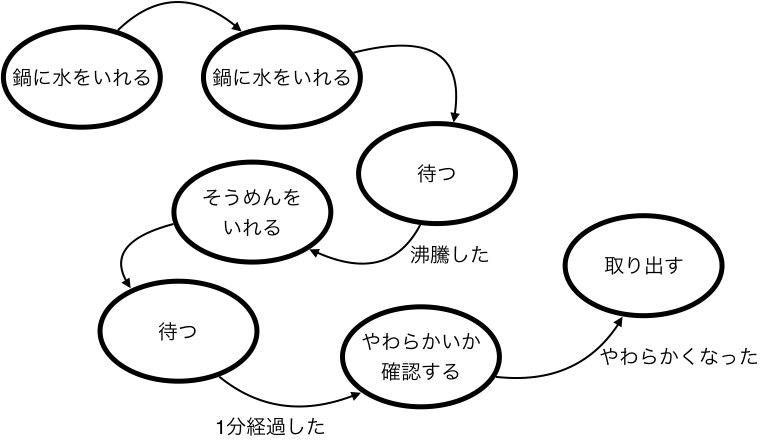
\includegraphics[width=.6\textwidth]{chapter05_figures/statemachine_example.png}
  \end{center}  
  \caption{そうめんを茹でる流れをステートマシン的に表現してみた例.\label{fig:statemachine_example}}
 \end{figure}


ステート・マシンとは,処理を「状態」と「状態遷移」で抽象化した概念です.列挙された状態を定義された状態遷移に従って順々にたどっていくことで所望の処理が実現できます.各状態での処理を定義することで,逐次的な処理をステート・マシンを使って記述できます.

\subsection{ハードウェア・プログラミングと相性の良いステート・マシン}
ステート・マシンをハードウェア・プログラミングで実装するのは意外と簡単です.そうめんを茹でる手順をハードウェア記述言語の一つであるVHDLで記述した擬似コードを示します.
各状態を\verb|std_logic_vector|型の変数stateで管理しています.stateの値が各状態に対応しています.変数stateをクロックごとに参照し,その時点で実行すべき処理を判断します.各状態では,次の状態に遷移するための条件判断と,遷移のための状態変数の更新を行います.

\begin{figure}[H]
\begin{quote}
\begin{Verbatim}[frame=single, numbers=left, baselinestretch=0.8]
---------------------------------------------------------
-- そうめんをゆでるステートマシンの擬似コード
---------------------------------------------------------
architecture RTL of somen

  signal state : std_logic_vector(2 downto 0) := (others => '0');

  process(clk)
  begin
    if rising_edge(clk) then
      case conv_integer(state) -- 変数「state」によって状態の場合分けをする
        when 0 =>
          鍋に水をいれる
          state <= conv_std_logic_vector(1, 3);
        when 1 =>
          鍋を火をかける
          state <= conv_std_logic_vector(2, 3);
        when 2 =>
          if 水が湧いたか? = true then
            state <= conv_std_logic_vector(3, 3);
          end if;
        when 3 =>
          そうめんをいれる
          state <= conv_std_logic_vector(4, 3);
        when 4 =>
          if 時間 = 1分 then
            state <= conv_std_logic_vector(5, 3);
          end if;
        when 5 =>
          if やわらかさが十分か? = true then
            state <= conv_std_logic_vector(6, 3);
          end if;
        when 6 =>
          -- おしまい
        when others => -- 「上記以外のその他」に相当.これで,全条件を列挙できた.
          null;
      end case; 
    end if;
  end process;

end RTL;
\end{Verbatim}
\end{quote}
\end{figure}

ところで,リスト1のコードには,0,1,2,...という状態を識別するための番号が振られています.これらの値に意味はなく,単にほかと区別するために便宜的に付けられたマジック・ナンバです.マジック・ナンバはコードの可読性を下げ,後の変更を加えづらくします.ソフトウェアでもマジック・ナンバは忌み嫌われるように,ハードウェア・プログラミングでもできれば避けたいものです.

VHDLでは自分で型を定義することで,Verilogではdefineやlocalparamを使って値に名前を付けることで,ソース・コードからマジック・ナンバを取り除くことができます.VHDLで状態を表す型を定義して,マジック・ナンバをなくした例が次の通りです.

\begin{figure}[H]
\begin{quote}
\begin{Verbatim}[frame=single, numbers=left, baselinestretch=0.8]
---------------------------------------------------------
-- そうめんをゆでるステートマシンの擬似コード
-- 状態変数のための型を定義しマジックナンバをなくしたバージョン
---------------------------------------------------------
architecture RTL of somen

  -- 状態を表わす型を定義する.これは,enumのような列挙型に相当.
  type StateType is (WATER, FIRE, HOT_WATER, PUT_SOMEN, WAIT_A_MIN, BOIL, FIN)
  signal state : StateType := WATER;

  process(clk)
  begin
    if rising_edge(clk) then
      case conv_integer(state)
        when WATER =>
          鍋に水をいれる
          state <= FIRE;
        when FIRE =>
          鍋を火をかける
          state <= HOT_WATER;
        when HOT_WATER =>
          if "水が湧いたか? = true" then
            state <= PUT_SOMEN;
          end if;
        when PUT_SOMEN =>
          そうめんをいれる
          state <= WAIT_A_MIN;
        when WAIT_A_MIN =>
          if 時間 = 1分 then
            state <= BOIL
          end if;
        when BOIL =>
          if やわらかさが十分か? = true then
            state <= conv_std_logic_vector(6, 3);
          end if;
        when FIN =>
          -- おしまい
        when others =>
          null;
      end case; 
    end if;
  end process;

end RTL;
\end{Verbatim}
\end{quote}
\end{figure}

次のリストを参考に,ステートマシンを利用したハードウェアを設計し,動作をシミュレーションとILAで確認してみてください.

\begin{figure}[H]
\begin{quote}
\begin{Verbatim}[frame=single, numbers=left, baselinestretch=0.6]
library ieee;
use ieee.std_logic_1164.all;
use ieee.numeric_std.all;

entity stmt_test is
  port ( clk : in std_logic;
         a,b : in std_logic;
         led : out std_logic_vector(2 downto 0)
       );
end stmt_test;

architecture RTL of stmt_test is
  attribute mark_debug : string;

  signal led_i : std_logic_vector(2 downto 0) := (others => '0');
  attribute mark_debug of led_i : signal is "true";

  type StateType is (BLACK, RED, GREEN, BLUE);
  signal state : StateType := BLACK;

  signal a_d, b_d : std_logic := '0';
  signal a_rising, b_rising : std_logic := '0';

begin

  led <= led_i;
  a_rising <= '1' when a_d = '0' and a = '1' else '0';
  b_rising <= '1' when b_d = '0' and b = '1' else '0';
  
  process(clk)
  begin
    if rising_edge(clk) then
      a_d <= a;
      b_d <= b;

      case state is
      when BLACK =>
        led_i <= "000";
        if a_rising = '1' then
          state <= RED;
        elsif b_rising = '1' then
          state <= BLUE;
        end if;
      when RED =>
        led_i <= "001";
        if a_rising = '1' then
          state <= GREEN;
        elsif b_rising = '1' then
          state <= BLACK;
        end if;
      when GREEN =>
        led_i <= "010";
        if a_rising = '1' then
          state <= BLUE;
        elsif b_rising = '1' then
          state <= RED;
        end if;
      when BLUE =>
        led_i <= "100";
        if a_rising = '1' then
          state <= BLACK;
        elsif b_rising = '1' then
          state <= GREEN;
        end if;
      when others =>
        led_i <= "000";
        state <= BLACK;
     end case;
    end if;
  end process;
end RTL;
\end{Verbatim}
\end{quote}
\end{figure}

\section*{参考文献}
\begin{enumerate}
 \item George Marsaglia, "Xorshift RNGs", The Florida State University, \url{http://www.jstatsoft.org/v08/i14}
\end{enumerate}

\end{document}
